
    




    
\documentclass[11pt]{article}

    
    \usepackage[breakable]{tcolorbox}
    \tcbset{nobeforeafter} % prevents tcolorboxes being placing in paragraphs
    \usepackage{float}
    \floatplacement{figure}{H} % forces figures to be placed at the correct location
    
    \usepackage[T1]{fontenc}
    % Nicer default font (+ math font) than Computer Modern for most use cases
    \usepackage{mathpazo}

    % Basic figure setup, for now with no caption control since it's done
    % automatically by Pandoc (which extracts ![](path) syntax from Markdown).
    \usepackage{graphicx}
    % We will generate all images so they have a width \maxwidth. This means
    % that they will get their normal width if they fit onto the page, but
    % are scaled down if they would overflow the margins.
    \makeatletter
    \def\maxwidth{\ifdim\Gin@nat@width>\linewidth\linewidth
    \else\Gin@nat@width\fi}
    \makeatother
    \let\Oldincludegraphics\includegraphics
    % Set max figure width to be 80% of text width, for now hardcoded.
    \renewcommand{\includegraphics}[1]{\Oldincludegraphics[width=.8\maxwidth]{#1}}
    % Ensure that by default, figures have no caption (until we provide a
    % proper Figure object with a Caption API and a way to capture that
    % in the conversion process - todo).
    \usepackage{caption}
    \DeclareCaptionLabelFormat{nolabel}{}
    \captionsetup{labelformat=nolabel}

    \usepackage{adjustbox} % Used to constrain images to a maximum size 
    \usepackage{xcolor} % Allow colors to be defined
    \usepackage{enumerate} % Needed for markdown enumerations to work
    \usepackage{geometry} % Used to adjust the document margins
    \usepackage{amsmath} % Equations
    \usepackage{amssymb} % Equations
    \usepackage{textcomp} % defines textquotesingle
    % Hack from http://tex.stackexchange.com/a/47451/13684:
    \AtBeginDocument{%
        \def\PYZsq{\textquotesingle}% Upright quotes in Pygmentized code
    }
    \usepackage{upquote} % Upright quotes for verbatim code
    \usepackage{eurosym} % defines \euro
    \usepackage[mathletters]{ucs} % Extended unicode (utf-8) support
    \usepackage[utf8x]{inputenc} % Allow utf-8 characters in the tex document
    \usepackage{fancyvrb} % verbatim replacement that allows latex
    \usepackage{grffile} % extends the file name processing of package graphics 
                         % to support a larger range 
    % The hyperref package gives us a pdf with properly built
    % internal navigation ('pdf bookmarks' for the table of contents,
    % internal cross-reference links, web links for URLs, etc.)
    \usepackage{hyperref}
    \usepackage{longtable} % longtable support required by pandoc >1.10
    \usepackage{booktabs}  % table support for pandoc > 1.12.2
    \usepackage[inline]{enumitem} % IRkernel/repr support (it uses the enumerate* environment)
    \usepackage[normalem]{ulem} % ulem is needed to support strikethroughs (\sout)
                                % normalem makes italics be italics, not underlines
    \usepackage{mathrsfs}
    

    
    % Colors for the hyperref package
    \definecolor{urlcolor}{rgb}{0,.145,.698}
    \definecolor{linkcolor}{rgb}{.71,0.21,0.01}
    \definecolor{citecolor}{rgb}{.12,.54,.11}

    % ANSI colors
    \definecolor{ansi-black}{HTML}{3E424D}
    \definecolor{ansi-black-intense}{HTML}{282C36}
    \definecolor{ansi-red}{HTML}{E75C58}
    \definecolor{ansi-red-intense}{HTML}{B22B31}
    \definecolor{ansi-green}{HTML}{00A250}
    \definecolor{ansi-green-intense}{HTML}{007427}
    \definecolor{ansi-yellow}{HTML}{DDB62B}
    \definecolor{ansi-yellow-intense}{HTML}{B27D12}
    \definecolor{ansi-blue}{HTML}{208FFB}
    \definecolor{ansi-blue-intense}{HTML}{0065CA}
    \definecolor{ansi-magenta}{HTML}{D160C4}
    \definecolor{ansi-magenta-intense}{HTML}{A03196}
    \definecolor{ansi-cyan}{HTML}{60C6C8}
    \definecolor{ansi-cyan-intense}{HTML}{258F8F}
    \definecolor{ansi-white}{HTML}{C5C1B4}
    \definecolor{ansi-white-intense}{HTML}{A1A6B2}
    \definecolor{ansi-default-inverse-fg}{HTML}{FFFFFF}
    \definecolor{ansi-default-inverse-bg}{HTML}{000000}

    % commands and environments needed by pandoc snippets
    % extracted from the output of `pandoc -s`
    \providecommand{\tightlist}{%
      \setlength{\itemsep}{0pt}\setlength{\parskip}{0pt}}
    \DefineVerbatimEnvironment{Highlighting}{Verbatim}{commandchars=\\\{\}}
    % Add ',fontsize=\small' for more characters per line
    \newenvironment{Shaded}{}{}
    \newcommand{\KeywordTok}[1]{\textcolor[rgb]{0.00,0.44,0.13}{\textbf{{#1}}}}
    \newcommand{\DataTypeTok}[1]{\textcolor[rgb]{0.56,0.13,0.00}{{#1}}}
    \newcommand{\DecValTok}[1]{\textcolor[rgb]{0.25,0.63,0.44}{{#1}}}
    \newcommand{\BaseNTok}[1]{\textcolor[rgb]{0.25,0.63,0.44}{{#1}}}
    \newcommand{\FloatTok}[1]{\textcolor[rgb]{0.25,0.63,0.44}{{#1}}}
    \newcommand{\CharTok}[1]{\textcolor[rgb]{0.25,0.44,0.63}{{#1}}}
    \newcommand{\StringTok}[1]{\textcolor[rgb]{0.25,0.44,0.63}{{#1}}}
    \newcommand{\CommentTok}[1]{\textcolor[rgb]{0.38,0.63,0.69}{\textit{{#1}}}}
    \newcommand{\OtherTok}[1]{\textcolor[rgb]{0.00,0.44,0.13}{{#1}}}
    \newcommand{\AlertTok}[1]{\textcolor[rgb]{1.00,0.00,0.00}{\textbf{{#1}}}}
    \newcommand{\FunctionTok}[1]{\textcolor[rgb]{0.02,0.16,0.49}{{#1}}}
    \newcommand{\RegionMarkerTok}[1]{{#1}}
    \newcommand{\ErrorTok}[1]{\textcolor[rgb]{1.00,0.00,0.00}{\textbf{{#1}}}}
    \newcommand{\NormalTok}[1]{{#1}}
    
    % Additional commands for more recent versions of Pandoc
    \newcommand{\ConstantTok}[1]{\textcolor[rgb]{0.53,0.00,0.00}{{#1}}}
    \newcommand{\SpecialCharTok}[1]{\textcolor[rgb]{0.25,0.44,0.63}{{#1}}}
    \newcommand{\VerbatimStringTok}[1]{\textcolor[rgb]{0.25,0.44,0.63}{{#1}}}
    \newcommand{\SpecialStringTok}[1]{\textcolor[rgb]{0.73,0.40,0.53}{{#1}}}
    \newcommand{\ImportTok}[1]{{#1}}
    \newcommand{\DocumentationTok}[1]{\textcolor[rgb]{0.73,0.13,0.13}{\textit{{#1}}}}
    \newcommand{\AnnotationTok}[1]{\textcolor[rgb]{0.38,0.63,0.69}{\textbf{\textit{{#1}}}}}
    \newcommand{\CommentVarTok}[1]{\textcolor[rgb]{0.38,0.63,0.69}{\textbf{\textit{{#1}}}}}
    \newcommand{\VariableTok}[1]{\textcolor[rgb]{0.10,0.09,0.49}{{#1}}}
    \newcommand{\ControlFlowTok}[1]{\textcolor[rgb]{0.00,0.44,0.13}{\textbf{{#1}}}}
    \newcommand{\OperatorTok}[1]{\textcolor[rgb]{0.40,0.40,0.40}{{#1}}}
    \newcommand{\BuiltInTok}[1]{{#1}}
    \newcommand{\ExtensionTok}[1]{{#1}}
    \newcommand{\PreprocessorTok}[1]{\textcolor[rgb]{0.74,0.48,0.00}{{#1}}}
    \newcommand{\AttributeTok}[1]{\textcolor[rgb]{0.49,0.56,0.16}{{#1}}}
    \newcommand{\InformationTok}[1]{\textcolor[rgb]{0.38,0.63,0.69}{\textbf{\textit{{#1}}}}}
    \newcommand{\WarningTok}[1]{\textcolor[rgb]{0.38,0.63,0.69}{\textbf{\textit{{#1}}}}}
    
    
    % Define a nice break command that doesn't care if a line doesn't already
    % exist.
    \def\br{\hspace*{\fill} \\* }
    % Math Jax compatibility definitions
    \def\gt{>}
    \def\lt{<}
    \let\Oldtex\TeX
    \let\Oldlatex\LaTeX
    \renewcommand{\TeX}{\textrm{\Oldtex}}
    \renewcommand{\LaTeX}{\textrm{\Oldlatex}}
    % Document parameters
    % Document title
    \title{	
	\normalfont\normalsize
	\textsc{ 5CL}\ % Your university, school and/or department name(s)
	\vspace{25pt} % Whitespace
	\rule{\linewidth}{0.5pt}\ % Thin top horizontal rule
	\vspace{20pt} % Whitespace
	{\huge Lab 6: Atomic Spectra}\ % The assignment title
	\vspace{12pt} % Whitespace
	\rule{\linewidth}{2pt}\ % Thick bottom horizontal rule
	\vspace{12pt} % Whitespace
}

\author{\LARGE Daniel Geisz \& Heidi Hu} % Your name

\date{\normalsize\today}
    
    
    
    
    
% Pygments definitions
\makeatletter
\def\PY@reset{\let\PY@it=\relax \let\PY@bf=\relax%
    \let\PY@ul=\relax \let\PY@tc=\relax%
    \let\PY@bc=\relax \let\PY@ff=\relax}
\def\PY@tok#1{\csname PY@tok@#1\endcsname}
\def\PY@toks#1+{\ifx\relax#1\empty\else%
    \PY@tok{#1}\expandafter\PY@toks\fi}
\def\PY@do#1{\PY@bc{\PY@tc{\PY@ul{%
    \PY@it{\PY@bf{\PY@ff{#1}}}}}}}
\def\PY#1#2{\PY@reset\PY@toks#1+\relax+\PY@do{#2}}

\expandafter\def\csname PY@tok@w\endcsname{\def\PY@tc##1{\textcolor[rgb]{0.73,0.73,0.73}{##1}}}
\expandafter\def\csname PY@tok@c\endcsname{\let\PY@it=\textit\def\PY@tc##1{\textcolor[rgb]{0.25,0.50,0.50}{##1}}}
\expandafter\def\csname PY@tok@cp\endcsname{\def\PY@tc##1{\textcolor[rgb]{0.74,0.48,0.00}{##1}}}
\expandafter\def\csname PY@tok@k\endcsname{\let\PY@bf=\textbf\def\PY@tc##1{\textcolor[rgb]{0.00,0.50,0.00}{##1}}}
\expandafter\def\csname PY@tok@kp\endcsname{\def\PY@tc##1{\textcolor[rgb]{0.00,0.50,0.00}{##1}}}
\expandafter\def\csname PY@tok@kt\endcsname{\def\PY@tc##1{\textcolor[rgb]{0.69,0.00,0.25}{##1}}}
\expandafter\def\csname PY@tok@o\endcsname{\def\PY@tc##1{\textcolor[rgb]{0.40,0.40,0.40}{##1}}}
\expandafter\def\csname PY@tok@ow\endcsname{\let\PY@bf=\textbf\def\PY@tc##1{\textcolor[rgb]{0.67,0.13,1.00}{##1}}}
\expandafter\def\csname PY@tok@nb\endcsname{\def\PY@tc##1{\textcolor[rgb]{0.00,0.50,0.00}{##1}}}
\expandafter\def\csname PY@tok@nf\endcsname{\def\PY@tc##1{\textcolor[rgb]{0.00,0.00,1.00}{##1}}}
\expandafter\def\csname PY@tok@nc\endcsname{\let\PY@bf=\textbf\def\PY@tc##1{\textcolor[rgb]{0.00,0.00,1.00}{##1}}}
\expandafter\def\csname PY@tok@nn\endcsname{\let\PY@bf=\textbf\def\PY@tc##1{\textcolor[rgb]{0.00,0.00,1.00}{##1}}}
\expandafter\def\csname PY@tok@ne\endcsname{\let\PY@bf=\textbf\def\PY@tc##1{\textcolor[rgb]{0.82,0.25,0.23}{##1}}}
\expandafter\def\csname PY@tok@nv\endcsname{\def\PY@tc##1{\textcolor[rgb]{0.10,0.09,0.49}{##1}}}
\expandafter\def\csname PY@tok@no\endcsname{\def\PY@tc##1{\textcolor[rgb]{0.53,0.00,0.00}{##1}}}
\expandafter\def\csname PY@tok@nl\endcsname{\def\PY@tc##1{\textcolor[rgb]{0.63,0.63,0.00}{##1}}}
\expandafter\def\csname PY@tok@ni\endcsname{\let\PY@bf=\textbf\def\PY@tc##1{\textcolor[rgb]{0.60,0.60,0.60}{##1}}}
\expandafter\def\csname PY@tok@na\endcsname{\def\PY@tc##1{\textcolor[rgb]{0.49,0.56,0.16}{##1}}}
\expandafter\def\csname PY@tok@nt\endcsname{\let\PY@bf=\textbf\def\PY@tc##1{\textcolor[rgb]{0.00,0.50,0.00}{##1}}}
\expandafter\def\csname PY@tok@nd\endcsname{\def\PY@tc##1{\textcolor[rgb]{0.67,0.13,1.00}{##1}}}
\expandafter\def\csname PY@tok@s\endcsname{\def\PY@tc##1{\textcolor[rgb]{0.73,0.13,0.13}{##1}}}
\expandafter\def\csname PY@tok@sd\endcsname{\let\PY@it=\textit\def\PY@tc##1{\textcolor[rgb]{0.73,0.13,0.13}{##1}}}
\expandafter\def\csname PY@tok@si\endcsname{\let\PY@bf=\textbf\def\PY@tc##1{\textcolor[rgb]{0.73,0.40,0.53}{##1}}}
\expandafter\def\csname PY@tok@se\endcsname{\let\PY@bf=\textbf\def\PY@tc##1{\textcolor[rgb]{0.73,0.40,0.13}{##1}}}
\expandafter\def\csname PY@tok@sr\endcsname{\def\PY@tc##1{\textcolor[rgb]{0.73,0.40,0.53}{##1}}}
\expandafter\def\csname PY@tok@ss\endcsname{\def\PY@tc##1{\textcolor[rgb]{0.10,0.09,0.49}{##1}}}
\expandafter\def\csname PY@tok@sx\endcsname{\def\PY@tc##1{\textcolor[rgb]{0.00,0.50,0.00}{##1}}}
\expandafter\def\csname PY@tok@m\endcsname{\def\PY@tc##1{\textcolor[rgb]{0.40,0.40,0.40}{##1}}}
\expandafter\def\csname PY@tok@gh\endcsname{\let\PY@bf=\textbf\def\PY@tc##1{\textcolor[rgb]{0.00,0.00,0.50}{##1}}}
\expandafter\def\csname PY@tok@gu\endcsname{\let\PY@bf=\textbf\def\PY@tc##1{\textcolor[rgb]{0.50,0.00,0.50}{##1}}}
\expandafter\def\csname PY@tok@gd\endcsname{\def\PY@tc##1{\textcolor[rgb]{0.63,0.00,0.00}{##1}}}
\expandafter\def\csname PY@tok@gi\endcsname{\def\PY@tc##1{\textcolor[rgb]{0.00,0.63,0.00}{##1}}}
\expandafter\def\csname PY@tok@gr\endcsname{\def\PY@tc##1{\textcolor[rgb]{1.00,0.00,0.00}{##1}}}
\expandafter\def\csname PY@tok@ge\endcsname{\let\PY@it=\textit}
\expandafter\def\csname PY@tok@gs\endcsname{\let\PY@bf=\textbf}
\expandafter\def\csname PY@tok@gp\endcsname{\let\PY@bf=\textbf\def\PY@tc##1{\textcolor[rgb]{0.00,0.00,0.50}{##1}}}
\expandafter\def\csname PY@tok@go\endcsname{\def\PY@tc##1{\textcolor[rgb]{0.53,0.53,0.53}{##1}}}
\expandafter\def\csname PY@tok@gt\endcsname{\def\PY@tc##1{\textcolor[rgb]{0.00,0.27,0.87}{##1}}}
\expandafter\def\csname PY@tok@err\endcsname{\def\PY@bc##1{\setlength{\fboxsep}{0pt}\fcolorbox[rgb]{1.00,0.00,0.00}{1,1,1}{\strut ##1}}}
\expandafter\def\csname PY@tok@kc\endcsname{\let\PY@bf=\textbf\def\PY@tc##1{\textcolor[rgb]{0.00,0.50,0.00}{##1}}}
\expandafter\def\csname PY@tok@kd\endcsname{\let\PY@bf=\textbf\def\PY@tc##1{\textcolor[rgb]{0.00,0.50,0.00}{##1}}}
\expandafter\def\csname PY@tok@kn\endcsname{\let\PY@bf=\textbf\def\PY@tc##1{\textcolor[rgb]{0.00,0.50,0.00}{##1}}}
\expandafter\def\csname PY@tok@kr\endcsname{\let\PY@bf=\textbf\def\PY@tc##1{\textcolor[rgb]{0.00,0.50,0.00}{##1}}}
\expandafter\def\csname PY@tok@bp\endcsname{\def\PY@tc##1{\textcolor[rgb]{0.00,0.50,0.00}{##1}}}
\expandafter\def\csname PY@tok@fm\endcsname{\def\PY@tc##1{\textcolor[rgb]{0.00,0.00,1.00}{##1}}}
\expandafter\def\csname PY@tok@vc\endcsname{\def\PY@tc##1{\textcolor[rgb]{0.10,0.09,0.49}{##1}}}
\expandafter\def\csname PY@tok@vg\endcsname{\def\PY@tc##1{\textcolor[rgb]{0.10,0.09,0.49}{##1}}}
\expandafter\def\csname PY@tok@vi\endcsname{\def\PY@tc##1{\textcolor[rgb]{0.10,0.09,0.49}{##1}}}
\expandafter\def\csname PY@tok@vm\endcsname{\def\PY@tc##1{\textcolor[rgb]{0.10,0.09,0.49}{##1}}}
\expandafter\def\csname PY@tok@sa\endcsname{\def\PY@tc##1{\textcolor[rgb]{0.73,0.13,0.13}{##1}}}
\expandafter\def\csname PY@tok@sb\endcsname{\def\PY@tc##1{\textcolor[rgb]{0.73,0.13,0.13}{##1}}}
\expandafter\def\csname PY@tok@sc\endcsname{\def\PY@tc##1{\textcolor[rgb]{0.73,0.13,0.13}{##1}}}
\expandafter\def\csname PY@tok@dl\endcsname{\def\PY@tc##1{\textcolor[rgb]{0.73,0.13,0.13}{##1}}}
\expandafter\def\csname PY@tok@s2\endcsname{\def\PY@tc##1{\textcolor[rgb]{0.73,0.13,0.13}{##1}}}
\expandafter\def\csname PY@tok@sh\endcsname{\def\PY@tc##1{\textcolor[rgb]{0.73,0.13,0.13}{##1}}}
\expandafter\def\csname PY@tok@s1\endcsname{\def\PY@tc##1{\textcolor[rgb]{0.73,0.13,0.13}{##1}}}
\expandafter\def\csname PY@tok@mb\endcsname{\def\PY@tc##1{\textcolor[rgb]{0.40,0.40,0.40}{##1}}}
\expandafter\def\csname PY@tok@mf\endcsname{\def\PY@tc##1{\textcolor[rgb]{0.40,0.40,0.40}{##1}}}
\expandafter\def\csname PY@tok@mh\endcsname{\def\PY@tc##1{\textcolor[rgb]{0.40,0.40,0.40}{##1}}}
\expandafter\def\csname PY@tok@mi\endcsname{\def\PY@tc##1{\textcolor[rgb]{0.40,0.40,0.40}{##1}}}
\expandafter\def\csname PY@tok@il\endcsname{\def\PY@tc##1{\textcolor[rgb]{0.40,0.40,0.40}{##1}}}
\expandafter\def\csname PY@tok@mo\endcsname{\def\PY@tc##1{\textcolor[rgb]{0.40,0.40,0.40}{##1}}}
\expandafter\def\csname PY@tok@ch\endcsname{\let\PY@it=\textit\def\PY@tc##1{\textcolor[rgb]{0.25,0.50,0.50}{##1}}}
\expandafter\def\csname PY@tok@cm\endcsname{\let\PY@it=\textit\def\PY@tc##1{\textcolor[rgb]{0.25,0.50,0.50}{##1}}}
\expandafter\def\csname PY@tok@cpf\endcsname{\let\PY@it=\textit\def\PY@tc##1{\textcolor[rgb]{0.25,0.50,0.50}{##1}}}
\expandafter\def\csname PY@tok@c1\endcsname{\let\PY@it=\textit\def\PY@tc##1{\textcolor[rgb]{0.25,0.50,0.50}{##1}}}
\expandafter\def\csname PY@tok@cs\endcsname{\let\PY@it=\textit\def\PY@tc##1{\textcolor[rgb]{0.25,0.50,0.50}{##1}}}

\def\PYZbs{\char`\\}
\def\PYZus{\char`\_}
\def\PYZob{\char`\{}
\def\PYZcb{\char`\}}
\def\PYZca{\char`\^}
\def\PYZam{\char`\&}
\def\PYZlt{\char`\<}
\def\PYZgt{\char`\>}
\def\PYZsh{\char`\#}
\def\PYZpc{\char`\%}
\def\PYZdl{\char`\$}
\def\PYZhy{\char`\-}
\def\PYZsq{\char`\'}
\def\PYZdq{\char`\"}
\def\PYZti{\char`\~}
% for compatibility with earlier versions
\def\PYZat{@}
\def\PYZlb{[}
\def\PYZrb{]}
\makeatother


    % For linebreaks inside Verbatim environment from package fancyvrb. 
    \makeatletter
        \newbox\Wrappedcontinuationbox 
        \newbox\Wrappedvisiblespacebox 
        \newcommand*\Wrappedvisiblespace {\textcolor{red}{\textvisiblespace}} 
        \newcommand*\Wrappedcontinuationsymbol {\textcolor{red}{\llap{\tiny$\m@th\hookrightarrow$}}} 
        \newcommand*\Wrappedcontinuationindent {3ex } 
        \newcommand*\Wrappedafterbreak {\kern\Wrappedcontinuationindent\copy\Wrappedcontinuationbox} 
        % Take advantage of the already applied Pygments mark-up to insert 
        % potential linebreaks for TeX processing. 
        %        {, <, #, %, $, ' and ": go to next line. 
        %        _, }, ^, &, >, - and ~: stay at end of broken line. 
        % Use of \textquotesingle for straight quote. 
        \newcommand*\Wrappedbreaksatspecials {% 
            \def\PYGZus{\discretionary{\char`\_}{\Wrappedafterbreak}{\char`\_}}% 
            \def\PYGZob{\discretionary{}{\Wrappedafterbreak\char`\{}{\char`\{}}% 
            \def\PYGZcb{\discretionary{\char`\}}{\Wrappedafterbreak}{\char`\}}}% 
            \def\PYGZca{\discretionary{\char`\^}{\Wrappedafterbreak}{\char`\^}}% 
            \def\PYGZam{\discretionary{\char`\&}{\Wrappedafterbreak}{\char`\&}}% 
            \def\PYGZlt{\discretionary{}{\Wrappedafterbreak\char`\<}{\char`\<}}% 
            \def\PYGZgt{\discretionary{\char`\>}{\Wrappedafterbreak}{\char`\>}}% 
            \def\PYGZsh{\discretionary{}{\Wrappedafterbreak\char`\#}{\char`\#}}% 
            \def\PYGZpc{\discretionary{}{\Wrappedafterbreak\char`\%}{\char`\%}}% 
            \def\PYGZdl{\discretionary{}{\Wrappedafterbreak\char`\$}{\char`\$}}% 
            \def\PYGZhy{\discretionary{\char`\-}{\Wrappedafterbreak}{\char`\-}}% 
            \def\PYGZsq{\discretionary{}{\Wrappedafterbreak\textquotesingle}{\textquotesingle}}% 
            \def\PYGZdq{\discretionary{}{\Wrappedafterbreak\char`\"}{\char`\"}}% 
            \def\PYGZti{\discretionary{\char`\~}{\Wrappedafterbreak}{\char`\~}}% 
        } 
        % Some characters . , ; ? ! / are not pygmentized. 
        % This macro makes them "active" and they will insert potential linebreaks 
        \newcommand*\Wrappedbreaksatpunct {% 
            \lccode`\~`\.\lowercase{\def~}{\discretionary{\hbox{\char`\.}}{\Wrappedafterbreak}{\hbox{\char`\.}}}% 
            \lccode`\~`\,\lowercase{\def~}{\discretionary{\hbox{\char`\,}}{\Wrappedafterbreak}{\hbox{\char`\,}}}% 
            \lccode`\~`\;\lowercase{\def~}{\discretionary{\hbox{\char`\;}}{\Wrappedafterbreak}{\hbox{\char`\;}}}% 
            \lccode`\~`\:\lowercase{\def~}{\discretionary{\hbox{\char`\:}}{\Wrappedafterbreak}{\hbox{\char`\:}}}% 
            \lccode`\~`\?\lowercase{\def~}{\discretionary{\hbox{\char`\?}}{\Wrappedafterbreak}{\hbox{\char`\?}}}% 
            \lccode`\~`\!\lowercase{\def~}{\discretionary{\hbox{\char`\!}}{\Wrappedafterbreak}{\hbox{\char`\!}}}% 
            \lccode`\~`\/\lowercase{\def~}{\discretionary{\hbox{\char`\/}}{\Wrappedafterbreak}{\hbox{\char`\/}}}% 
            \catcode`\.\active
            \catcode`\,\active 
            \catcode`\;\active
            \catcode`\:\active
            \catcode`\?\active
            \catcode`\!\active
            \catcode`\/\active 
            \lccode`\~`\~ 	
        }
    \makeatother

    \let\OriginalVerbatim=\Verbatim
    \makeatletter
    \renewcommand{\Verbatim}[1][1]{%
        %\parskip\z@skip
        \sbox\Wrappedcontinuationbox {\Wrappedcontinuationsymbol}%
        \sbox\Wrappedvisiblespacebox {\FV@SetupFont\Wrappedvisiblespace}%
        \def\FancyVerbFormatLine ##1{\hsize\linewidth
            \vtop{\raggedright\hyphenpenalty\z@\exhyphenpenalty\z@
                \doublehyphendemerits\z@\finalhyphendemerits\z@
                \strut ##1\strut}%
        }%
        % If the linebreak is at a space, the latter will be displayed as visible
        % space at end of first line, and a continuation symbol starts next line.
        % Stretch/shrink are however usually zero for typewriter font.
        \def\FV@Space {%
            \nobreak\hskip\z@ plus\fontdimen3\font minus\fontdimen4\font
            \discretionary{\copy\Wrappedvisiblespacebox}{\Wrappedafterbreak}
            {\kern\fontdimen2\font}%
        }%
        
        % Allow breaks at special characters using \PYG... macros.
        \Wrappedbreaksatspecials
        % Breaks at punctuation characters . , ; ? ! and / need catcode=\active 	
        \OriginalVerbatim[#1,codes*=\Wrappedbreaksatpunct]%
    }
    \makeatother

    % Exact colors from NB
    \definecolor{incolor}{HTML}{303F9F}
    \definecolor{outcolor}{HTML}{D84315}
    \definecolor{cellborder}{HTML}{CFCFCF}
    \definecolor{cellbackground}{HTML}{F7F7F7}
    
    % prompt
    \newcommand{\prompt}[4]{
        \llap{{\color{#2}[#3]: #4}}\vspace{-1.25em}
    }
    

    
    % Prevent overflowing lines due to hard-to-break entities
    \sloppy 
    % Setup hyperref package
    \hypersetup{
      breaklinks=true,  % so long urls are correctly broken across lines
      colorlinks=true,
      urlcolor=urlcolor,
      linkcolor=linkcolor,
      citecolor=citecolor,
      }
    % Slightly bigger margins than the latex defaults
    
    \geometry{verbose,tmargin=1in,bmargin=1in,lmargin=1in,rmargin=1in}
    
    

    \begin{document}
    
    
    \maketitle
    
    

    
    \hypertarget{experiment-2---the-bohring-world-of-hydrogen}{%
\section{Experiment 2 - The Bohring World of
Hydrogen}\label{experiment-2---the-bohring-world-of-hydrogen}}

\hypertarget{objective}{%
\subsection{Objective:}\label{objective}}

The purpose of this experiment is to observe and measure the Balmer
series of Hydrogen and use our data to find the Rydberg constant.

\hypertarget{method}{%
\subsection{Method:}\label{method}}

Setup the materials according to section 1.1 of the lab manual with the
discharge tube behind the spectrometer scale, but use the hydrogen tube
instead of the helium tube.

By looking through the grating we were able to observe the spectrum of
helium against the spectrometer scale. To measure the wavelength
\(\lambda\) of a given spectral line, we measured the distance between
the central maximum and the spectral line as viewed on the spectrometer
scale, and we measured the distance between the diffraction grating and
the spectrometer scale. We let \(a\) denote the distance between the
central maximum and the spectral line, and we let \(b\) denote the
distance between the diffraction grating and the spectrometer scale.
Finally we let \(D\) represent the slit density of the diffraction
grating, which we determined in experiment 1.

Using standard theory, we therefore have the following relation:

\[ \lambda = \frac{\sin\left(\tan^{-1}\left(\frac{a}{b}\right)\right)}{D} = \frac{a}{D\cdot \sqrt{a^2 + b^2}}\]

This has the following equation for error propagation:

\[\delta\lambda = \sqrt{\dfrac{\left((a^{3} + b^{2}a)\frac{\delta D}{D}\right)^{2} + (b^{2}\delta a)^{2} + (ab\delta b)^{2}}{D^{2}(a^{2}+b^{2})^{3}}}\]

Finally, in order to find the energy level transitions each spectral
line of hydrogen corresponded to, we compared our data with the accepted
values, which allowed us to determine \(n_i\), the energy level of the
electron before the transition, for each spectral line. Together our
knowledge of \(n_i\) and \(\lambda\) allows us to find the Rydberg
constant.

Finally, note that in Experiment 1, we measured \(D = 4873 \pm 49\)
slits per cm.

\hypertarget{answers-to-data-analysis-problems}{%
\subsection{Answers to Data Analysis
Problems:}\label{answers-to-data-analysis-problems}}

\begin{enumerate}
\def\labelenumi{\alph{enumi})}
\tightlist
\item
  Find the standard deviation and standard error for your multiple
  independent measurements for the position of the Helium D3 line from
  Experiment 1.1.
\end{enumerate}

The following data table corresponds to the data we took in Experiment
1.1. Here, ``Distance'' refers to the distance between the central
maximum and the D3 spectral line in centimeters.

    \begin{tcolorbox}[breakable, size=fbox, boxrule=1pt, pad at break*=1mm,colback=cellbackground, colframe=cellborder]
\prompt{In}{incolor}{7}{\hspace{4pt}}
\begin{Verbatim}[commandchars=\\\{\}]
\PY{n}{data1}
\end{Verbatim}
\end{tcolorbox}

            \begin{tcolorbox}[breakable, boxrule=.5pt, size=fbox, pad at break*=1mm, opacityfill=0]
\prompt{Out}{outcolor}{7}{\hspace{3.5pt}}
\begin{Verbatim}[commandchars=\\\{\}]
   Distance
0      22.2
1      22.1
2      22.2
3      22.3
\end{Verbatim}
\end{tcolorbox}
        
    The following script calculates the standard deviation and the standard
error of this data using the simple formulas for these quantities:

    \begin{tcolorbox}[breakable, size=fbox, boxrule=1pt, pad at break*=1mm,colback=cellbackground, colframe=cellborder]
\prompt{In}{incolor}{8}{\hspace{4pt}}
\begin{Verbatim}[commandchars=\\\{\}]
\PY{n}{std\PYZus{}dev} \PY{o}{=} \PY{p}{(}\PY{p}{(}\PY{n}{data1}\PY{o}{.}\PY{n}{Distance} \PY{o}{*}\PY{o}{*} \PY{l+m+mi}{2}\PY{p}{)}\PY{o}{.}\PY{n}{mean}\PY{p}{(}\PY{p}{)} \PY{o}{\PYZhy{}} \PY{p}{(}\PY{n}{data1}\PY{o}{.}\PY{n}{Distance}\PY{o}{.}\PY{n}{mean}\PY{p}{(}\PY{p}{)}\PY{p}{)}\PY{o}{*}\PY{o}{*}\PY{l+m+mi}{2}\PY{p}{)}\PY{o}{*}\PY{o}{*}\PY{l+m+mf}{0.5}
\PY{n}{std\PYZus{}err} \PY{o}{=} \PY{n}{std\PYZus{}dev} \PY{o}{/} \PY{l+m+mi}{2}

\PY{n+nb}{print}\PY{p}{(}\PY{l+s+s2}{\PYZdq{}}\PY{l+s+s2}{Standard Deviation: }\PY{l+s+s2}{\PYZdq{}}\PY{p}{,} \PY{n}{std\PYZus{}dev}\PY{p}{)}
\PY{n+nb}{print}\PY{p}{(}\PY{l+s+s2}{\PYZdq{}}\PY{l+s+s2}{Standard Error: }\PY{l+s+s2}{\PYZdq{}}\PY{p}{,} \PY{n}{std\PYZus{}err}\PY{p}{)}
\end{Verbatim}
\end{tcolorbox}

    \begin{Verbatim}[commandchars=\\\{\}]
Standard Deviation:  0.0707106781186226
Standard Error:  0.0353553390593113
\end{Verbatim}

    From this we see that:


\begin{gather}
Standard \; Deviation = 0.07\;\text{cm} \\
Standard \; Error = 0.04\;\text{cm}
\end{gather}

    \begin{enumerate}
\def\labelenumi{\alph{enumi})}
\tightlist
\item
  Make a scatter plot (with error bars) of
  \(\frac{1}{\lambda}\)-vs-\(\frac{1}{n^2_i}\).
\end{enumerate}

The following data table shows the data we took for this experiment.
Here, ``color'' refers to the color observed for the given spectral
line. Here ``a'' represents the quantity \(a\) from the Method section,
with units of centimeters. We take the standard error calculated in the
previous section to be the uncertainty of each measurement of ``a''.

    \begin{tcolorbox}[breakable, size=fbox, boxrule=1pt, pad at break*=1mm,colback=cellbackground, colframe=cellborder]
\prompt{In}{incolor}{9}{\hspace{4pt}}
\begin{Verbatim}[commandchars=\\\{\}]
\PY{n}{data2}
\end{Verbatim}
\end{tcolorbox}

            \begin{tcolorbox}[breakable, boxrule=.5pt, size=fbox, pad at break*=1mm, opacityfill=0]
\prompt{Out}{outcolor}{9}{\hspace{3.5pt}}
\begin{Verbatim}[commandchars=\\\{\}]
  Color     a
0  Blue  10.1
1  Teal  11.7
2   Red  16.5
\end{Verbatim}
\end{tcolorbox}
        
    For all data points, we found $b = 46.9 \pm 0.05$ cm. We are
therefore able to calculate \(\lambda\) for each color using the formula
in the method section. By matching our data to the predicted wavelengths
from the Rydberg formula, we are able to find the energy level
transition that each of data points corresponds to.

The following table compiles this information together. Here ``Color''
is the color of the spectral line observed, ``lambda'' is the wavelength
in nm, ``dlambda'' is the uncertainty in ``lambda'', and ``n'' is the
starting energy level that corresponds to the given data point.

    \begin{tcolorbox}[breakable, size=fbox, boxrule=1pt, pad at break*=1mm,colback=cellbackground, colframe=cellborder]
\prompt{In}{incolor}{10}{\hspace{4pt}}
\begin{Verbatim}[commandchars=\\\{\}]
\PY{n}{d3}
\end{Verbatim}
\end{tcolorbox}

            \begin{tcolorbox}[breakable, boxrule=.5pt, size=fbox, pad at break*=1mm, opacityfill=0]
\prompt{Out}{outcolor}{10}{\hspace{3.5pt}}
\begin{Verbatim}[commandchars=\\\{\}]
  Color      lambda    dlambda  n
0  Blue  432.024276  23.360825  5
1  Teal  496.714179  33.844799  4
2   Red  681.044669  81.119881  3
\end{Verbatim}
\end{tcolorbox}
        
    This final data table holds the same information as above, but now it
includes values of \(\frac{1}{\lambda}\). Here ``wl\^{}-1'' represents
\(\frac{1}{\lambda}\), and ``dwl\^{}-1'' is the associated uncertainty.
Note that both quantities have units of \(meters ^ {-1}\) to facilitate
later calculations. The other values in the above table remain the same.

    \begin{tcolorbox}[breakable, size=fbox, boxrule=1pt, pad at break*=1mm,colback=cellbackground, colframe=cellborder]
\prompt{In}{incolor}{21}{\hspace{4pt}}
\begin{Verbatim}[commandchars=\\\{\}]
\PY{n}{d4}
\end{Verbatim}
\end{tcolorbox}

            \begin{tcolorbox}[breakable, boxrule=.5pt, size=fbox, pad at break*=1mm, opacityfill=0]
\prompt{Out}{outcolor}{21}{\hspace{3.5pt}}
\begin{Verbatim}[commandchars=\\\{\}]
  Color         wl\^{}-1         dwl\^{}-1  n
0  Blue  2.314685e+06  125161.823875  5
1  Teal  2.013230e+06  137176.217853  4
2   Red  1.468332e+06  174894.483327  3
\end{Verbatim}
\end{tcolorbox}
        
    The following script plot values of \(\frac{1}{\lambda}\) against values
of \(\frac{1}{n ^2}\) with error bars.

    \begin{tcolorbox}[breakable, size=fbox, boxrule=1pt, pad at break*=1mm,colback=cellbackground, colframe=cellborder]
\prompt{In}{incolor}{24}{\hspace{4pt}}
\begin{Verbatim}[commandchars=\\\{\}]
\PY{n}{plt}\PY{o}{.}\PY{n}{errorbar}\PY{p}{(}\PY{p}{(}\PY{l+m+mi}{1} \PY{o}{/} \PY{n}{d4}\PY{o}{.}\PY{n}{n} \PY{o}{*}\PY{o}{*}\PY{l+m+mi}{2}\PY{p}{)} \PY{p}{,} \PY{n}{d4}\PY{p}{[}\PY{l+s+s1}{\PYZsq{}}\PY{l+s+s1}{wl\PYZca{}\PYZhy{}1}\PY{l+s+s1}{\PYZsq{}}\PY{p}{]}\PY{p}{,} \PY{n}{yerr}\PY{o}{=}\PY{n}{d4}\PY{p}{[}\PY{l+s+s1}{\PYZsq{}}\PY{l+s+s1}{dwl\PYZca{}\PYZhy{}1}\PY{l+s+s1}{\PYZsq{}}\PY{p}{]}\PY{p}{,} \PY{n}{fmt}\PY{o}{=}\PY{l+s+s1}{\PYZsq{}}\PY{l+s+s1}{.}\PY{l+s+s1}{\PYZsq{}}\PY{p}{)}
\PY{n}{plt}\PY{o}{.}\PY{n}{ylabel}\PY{p}{(}\PY{l+s+s2}{\PYZdq{}}\PY{l+s+s2}{1 / wavelength (m \PYZca{} \PYZhy{}1)}\PY{l+s+s2}{\PYZdq{}}\PY{p}{)}
\PY{n}{plt}\PY{o}{.}\PY{n}{title}\PY{p}{(}\PY{l+s+s2}{\PYZdq{}}\PY{l+s+s2}{Wavelength\PYZca{}\PYZhy{}1 vs n\PYZca{}\PYZhy{}2}\PY{l+s+s2}{\PYZdq{}}\PY{p}{)}
\PY{n}{plt}\PY{o}{.}\PY{n}{xlabel}\PY{p}{(}\PY{l+s+s2}{\PYZdq{}}\PY{l+s+s2}{1 / n\PYZca{}2}\PY{l+s+s2}{\PYZdq{}}\PY{p}{)}
\PY{n}{plt}\PY{o}{.}\PY{n}{show}\PY{p}{(}\PY{p}{)}
\end{Verbatim}
\end{tcolorbox}

    \begin{center}
    \adjustimage{max size={0.9\linewidth}{0.9\paperheight}}{output_12_0.png}
    \end{center}
    { \hspace*{\fill} \\}
    
    \begin{enumerate}
\def\labelenumi{\alph{enumi})}
\setcounter{enumi}{1}
\tightlist
\item
  Perform a regression to the linear function you found in Question
  Pre1(c) to find a best-fit value for the slope (with uncertainties).
\end{enumerate}

I will fit the data from the above scatter plot to a linear hypothesis,
\(\displaystyle \frac{1}{\lambda} = \hat{m}\left(\frac{1}{n^2}\right) + \hat{b}\)
using the weighted least squares method. The following script finds the
best fit parameters and their correspond uncertainties.

    \begin{tcolorbox}[breakable, size=fbox, boxrule=1pt, pad at break*=1mm,colback=cellbackground, colframe=cellborder]
\prompt{In}{incolor}{35}{\hspace{4pt}}
\begin{Verbatim}[commandchars=\\\{\}]
\PY{n}{w} \PY{o}{=} \PY{l+m+mi}{1} \PY{o}{/} \PY{p}{(}\PY{n}{d4}\PY{p}{[}\PY{l+s+s1}{\PYZsq{}}\PY{l+s+s1}{dwl\PYZca{}\PYZhy{}1}\PY{l+s+s1}{\PYZsq{}}\PY{p}{]} \PY{o}{*}\PY{o}{*} \PY{l+m+mi}{2}\PY{p}{)}
\PY{n}{y} \PY{o}{=} \PY{n}{d4}\PY{p}{[}\PY{l+s+s1}{\PYZsq{}}\PY{l+s+s1}{wl\PYZca{}\PYZhy{}1}\PY{l+s+s1}{\PYZsq{}}\PY{p}{]}
\PY{n}{x} \PY{o}{=} \PY{l+m+mi}{1} \PY{o}{/} \PY{p}{(}\PY{n}{d4}\PY{o}{.}\PY{n}{n} \PY{o}{*}\PY{o}{*} \PY{l+m+mi}{2}\PY{p}{)}

\PY{n}{denom} \PY{o}{=} \PY{p}{(}\PY{n}{w}\PY{o}{.}\PY{n}{sum}\PY{p}{(}\PY{p}{)} \PY{o}{*} \PY{p}{(}\PY{n}{w} \PY{o}{*} \PY{n}{x} \PY{o}{*} \PY{n}{x}\PY{p}{)}\PY{o}{.}\PY{n}{sum}\PY{p}{(}\PY{p}{)}\PY{p}{)} \PY{o}{\PYZhy{}} \PY{p}{(}\PY{p}{(}\PY{n}{w} \PY{o}{*} \PY{n}{x}\PY{p}{)}\PY{o}{.}\PY{n}{sum}\PY{p}{(}\PY{p}{)}\PY{p}{)} \PY{o}{*}\PY{o}{*}\PY{l+m+mi}{2}
\PY{n}{m} \PY{o}{=} \PY{p}{(}\PY{p}{(}\PY{n}{w}\PY{o}{.}\PY{n}{sum}\PY{p}{(}\PY{p}{)} \PY{o}{*} \PY{p}{(}\PY{n}{w} \PY{o}{*} \PY{n}{x} \PY{o}{*} \PY{n}{y}\PY{p}{)}\PY{o}{.}\PY{n}{sum}\PY{p}{(}\PY{p}{)}\PY{p}{)} \PY{o}{\PYZhy{}} \PY{p}{(}\PY{p}{(}\PY{n}{w} \PY{o}{*} \PY{n}{x}\PY{p}{)}\PY{o}{.}\PY{n}{sum}\PY{p}{(}\PY{p}{)}\PY{o}{*}\PY{p}{(}\PY{n}{w} \PY{o}{*} \PY{n}{y}\PY{p}{)}\PY{o}{.}\PY{n}{sum}\PY{p}{(}\PY{p}{)}\PY{p}{)}\PY{p}{)} \PY{o}{/} \PY{n}{denom}
\PY{n}{b} \PY{o}{=} \PY{p}{(}\PY{p}{(}\PY{n}{w} \PY{o}{*} \PY{n}{y}\PY{p}{)}\PY{o}{.}\PY{n}{sum}\PY{p}{(}\PY{p}{)} \PY{o}{\PYZhy{}} \PY{n}{m} \PY{o}{*} \PY{p}{(}\PY{n}{w} \PY{o}{*} \PY{n}{x}\PY{p}{)}\PY{o}{.}\PY{n}{sum}\PY{p}{(}\PY{p}{)}\PY{p}{)}\PY{o}{/} \PY{p}{(}\PY{n}{w}\PY{o}{.}\PY{n}{sum}\PY{p}{(}\PY{p}{)}\PY{p}{)}
\PY{n}{dm} \PY{o}{=} \PY{p}{(}\PY{n}{w}\PY{o}{.}\PY{n}{sum}\PY{p}{(}\PY{p}{)} \PY{o}{/} \PY{n}{denom}\PY{p}{)} \PY{o}{*}\PY{o}{*} \PY{l+m+mf}{0.5}
\PY{n}{db} \PY{o}{=} \PY{p}{(}\PY{p}{(}\PY{n}{w} \PY{o}{*} \PY{n}{x} \PY{o}{*} \PY{n}{x}\PY{p}{)}\PY{o}{.}\PY{n}{sum}\PY{p}{(}\PY{p}{)} \PY{o}{/} \PY{n}{denom}\PY{p}{)} \PY{o}{*}\PY{o}{*} \PY{l+m+mf}{0.5}
\PY{n+nb}{print}\PY{p}{(}\PY{l+s+s2}{\PYZdq{}}\PY{l+s+s2}{m: }\PY{l+s+s2}{\PYZdq{}}\PY{p}{,} \PY{n}{m}\PY{p}{,} \PY{l+s+s2}{\PYZdq{}}\PY{l+s+s2}{ +\PYZhy{} }\PY{l+s+s2}{\PYZdq{}}\PY{p}{,} \PY{n}{dm}\PY{p}{)}
\PY{n+nb}{print}\PY{p}{(}\PY{l+s+s2}{\PYZdq{}}\PY{l+s+s2}{b: }\PY{l+s+s2}{\PYZdq{}}\PY{p}{,} \PY{n}{b}\PY{p}{,} \PY{l+s+s2}{\PYZdq{}}\PY{l+s+s2}{ +\PYZhy{} }\PY{l+s+s2}{\PYZdq{}}\PY{p}{,} \PY{n}{db}\PY{p}{)}
\end{Verbatim}
\end{tcolorbox}

    \begin{Verbatim}[commandchars=\\\{\}]
m:  -11885121.339421667  +-  3023182.0882392027
b:  2777743.8993566805  +-  208710.35307243734
\end{Verbatim}

    Therefore we see that the best fit value of the slope is:

\[\boxed{\hat{m} = -1.19 \pm 0.30 \cdot 10^7 \; \text{meters} ^{-1}}\]

\begin{enumerate}
\def\labelenumi{\alph{enumi})}
\setcounter{enumi}{2}
\tightlist
\item
  Based on your fit values, determine the Rydberg constant (with
  uncertainty). Compare to the given value.
\end{enumerate}

Comparing to Equation (1) in the lab manual, we see that the Rydberg
constant is \(-\hat{m}\). Therefore performing a linear fit on our data
indicates that:

\[\boxed{ R = 1.19 \pm 0.30 \cdot 10^7 \; \text{meters} ^{-1}}\]

The accepted value for the Rydberg constant is
\(1.09 \cdot 10^7 \; \text{meters} ^{-1}\). Performing a simple
agreement test between this number and our experimental value yields
0.17, so we see that our experimentally determined value of the Rydberg
constant agrees with the accepted value.

    \hypertarget{experiment-3---mystery-tubes}{%
\section{Experiment 3 - Mystery
Tubes!}\label{experiment-3---mystery-tubes}}

\hypertarget{objective}{%
\subsection{Objective:}\label{objective}}

We will determine the gases in the unknown gas tubes by observing and
comparing their emission spectra to external references, measure
wavelengths of two of the most prominent spectral lines for each tube,
and verifying them with research results.

\hypertarget{method}{%
\subsection{Method:}\label{method}}

\begin{itemize}
\item
  Load tube B into the power supply and and set up the spectrometer as
  illustrated in the figure below to observe the emitted light.\\
  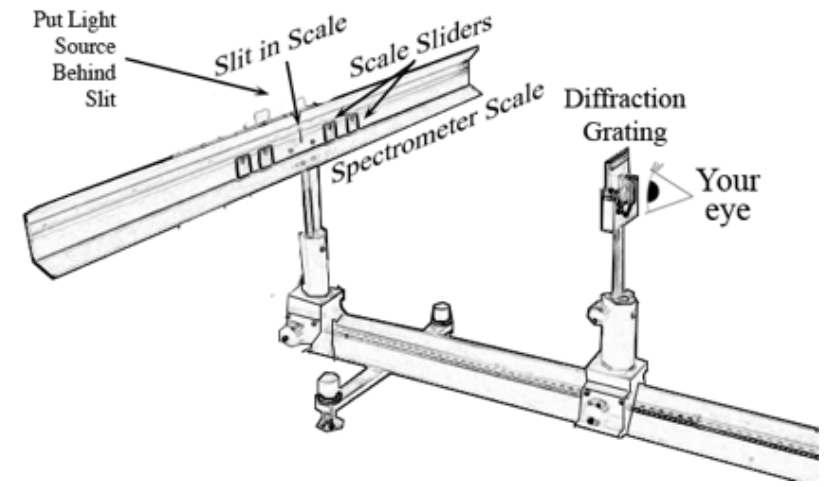
\includegraphics{setup.jpg}
\item
  Use the sliders to find the distance between the prominent spectral
  lines and the central maximum and record them.
\item
  Load tube C into power supply and repeat the procedures above.
\end{itemize}

Note that in the following analysis, we let the variable \(b\) equal the
distance between the diffraction grating and the spectrometer, and we
let the variable \(a\) represent the distance between the central
maximum and the prominent spectral line we're measuring. So then, to
collect data, we simply found \(a\) using the sliders and \(b\) using
the meter stick first for tube B, and then for tube C. We then used the
following equations to determine \(\lambda\), the wavelength of each
spectral line.

From theory we know that if θ is the angle between the central maximum
and the first fringe, d is the slit width of the diffraction grating,
and λ is the wavelength of the light being used, we have:

\[\lambda = dsin(\theta)\]

If \(D\) is the slit density of the diffraction grating, then
\(D = \frac{1}{d}\). Therefore, based on how the variables were defined,

\[ \theta = \tan ^{-1}\left(\frac{a}{b}\right)\]

So then,

\[\lambda = \dfrac{sin\theta}{D} = \dfrac{a}{D\sqrt{a^{2}+b^{2}}}\]\\
and therefore,\\
\[\delta_{\lambda} = \sqrt{\dfrac{((a^{3} + b^{2}a)\frac{\delta_{D}}{D})^{2} + (b^{2}\delta_{a})^{2} + (ab\delta_{b})^{2}}{D^{2}(a^{2}+b^{2})^{3}}}\]

Finally, it should be noted that in Experiment 1, we measured the slit
density D to be \(D = 4873\pm49 slits·cm^{-1}\).

    \hypertarget{data-analysis}{%
\subsection{Data Analysis:}\label{data-analysis}}

\hypertarget{determine-unknown-gas}{%
\subsubsection{Determine Unknown Gas}\label{determine-unknown-gas}}

The observed emission spectra of tube B 

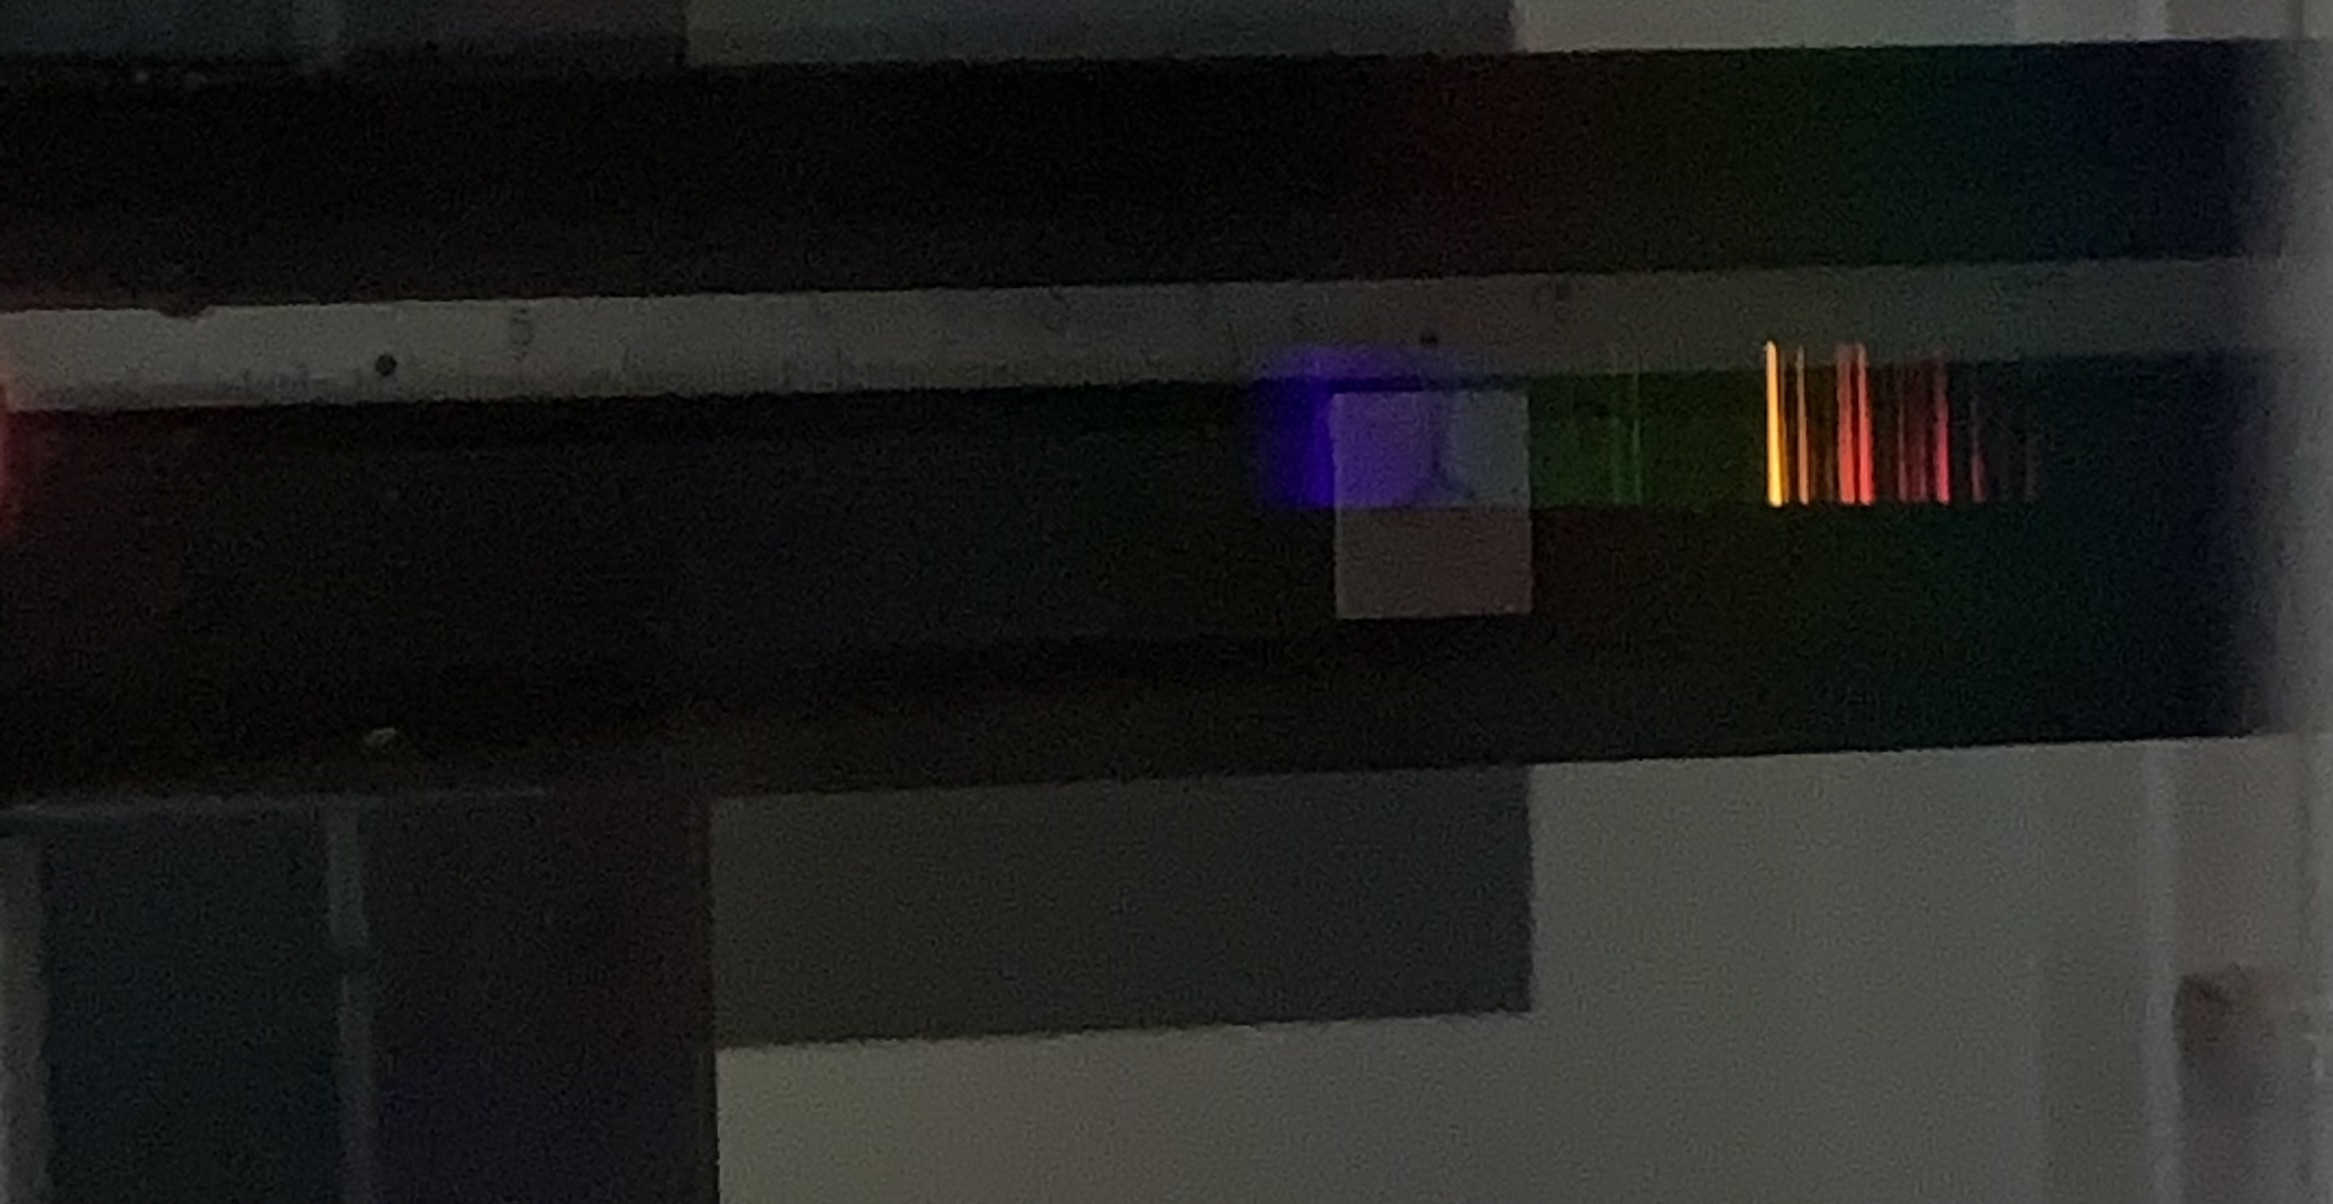
\includegraphics{BNeon.jpg} \\

The observed emission spectra of tube C 

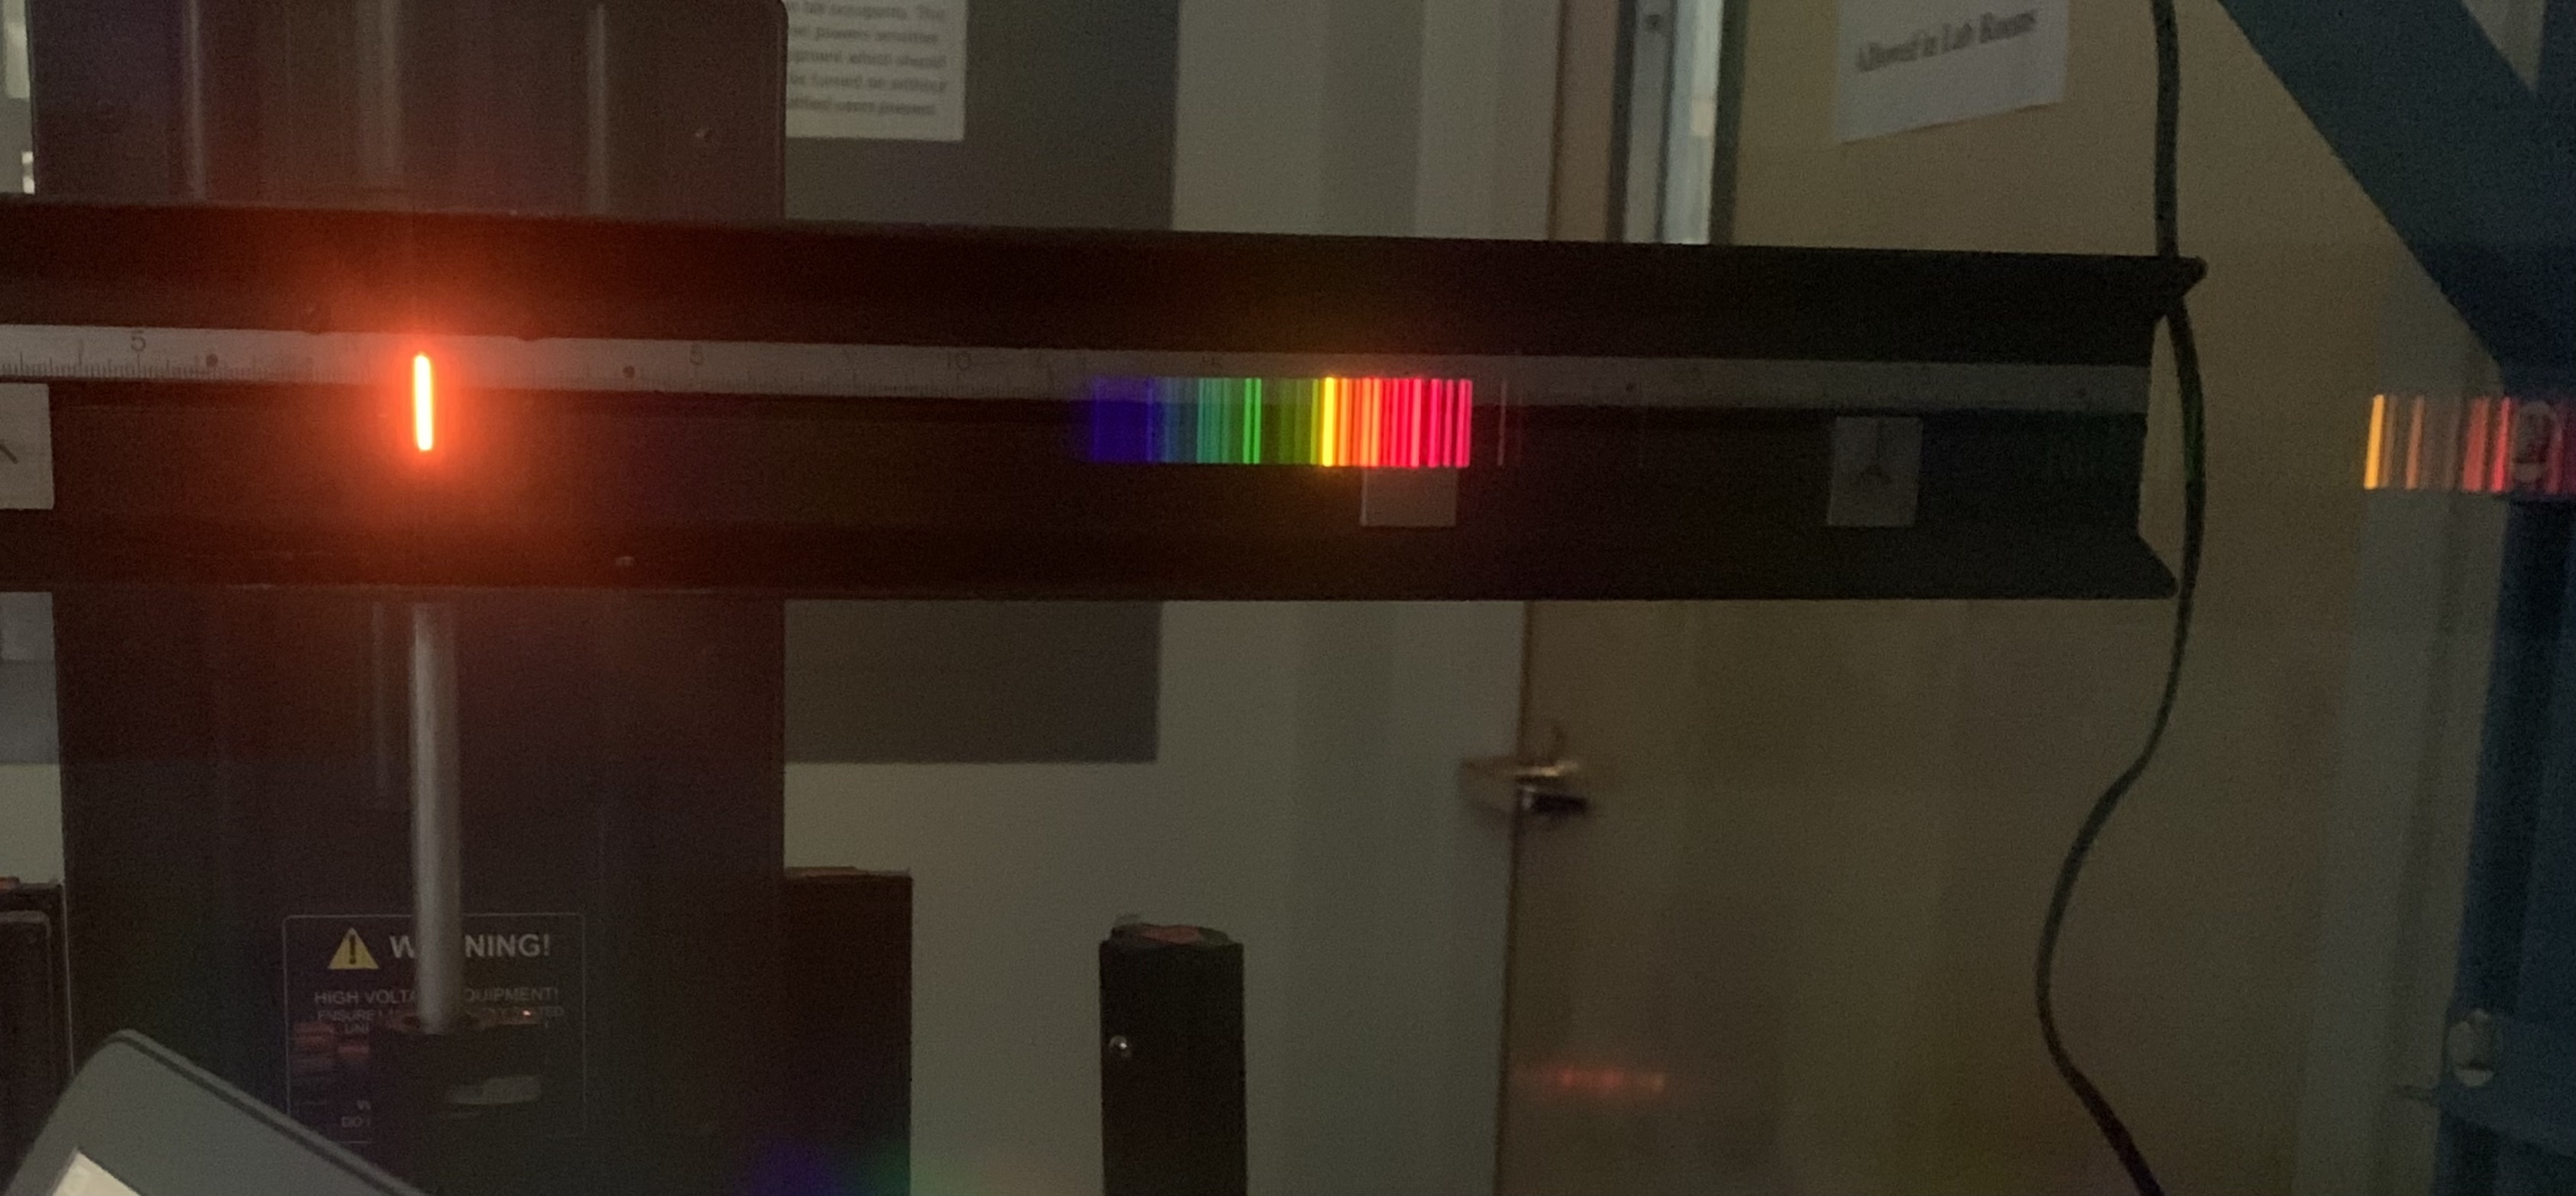
\includegraphics{CNitrogen.jpg}

The possibilities of these gases are given to be Nitrogen, Neon, and
Argon, with emission spectra below respectively from the source http://hyperphysics.phy-astr.gsu.edu/hbase/quantum/atspect.html

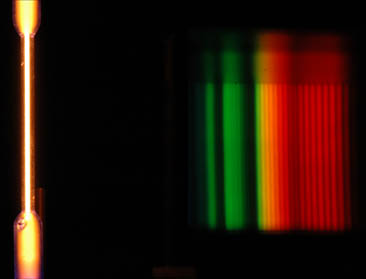
\includegraphics{standardNitrogen.jpg} \\

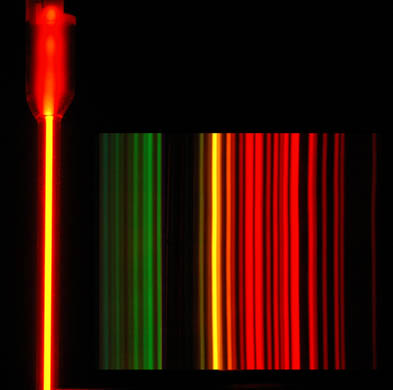
\includegraphics{standardNeon.jpg} \\

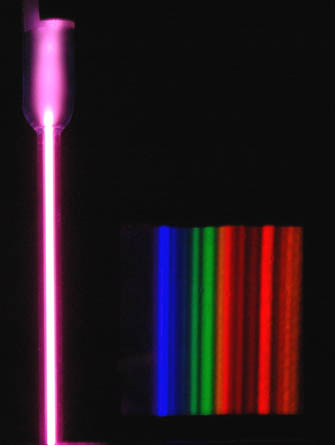
\includegraphics{standardArgon.jpg}

We observed that the emission spectra of B contains a bright yellow
line, followed by a series of bright orange and red lines, with a single
wide gap between green and yellow lines. The emission spectra of C
contains many bright green lines, a bright yellow line, followed by
bright red lines with two clear gaps within green lines. By comparing
these distinctive features with the provided emission spectrum, we were
able to deduce that tube B contains Neon and tube C contains Nitrogen.

\hypertarget{measure-prominent-wavelengths}{%
\subsubsection{Measure Prominent
Wavelengths}\label{measure-prominent-wavelengths}}

For tube B, we chose to measure the wavelengths of leading yellow and
orange lines; and for tube C, we chose to measure the wavelengths of
leading green and yellow lines.

In these tables, `a' stands for the distance between the spectral line
and central maximum with standard error of 0.04 for each measurement and
unit of cm; `b' stands for the distance between diffraction grating and
spectrometer with uncertainty of 0.05 for each measurement and unit of
cm.

    \begin{tcolorbox}[breakable, size=fbox, boxrule=1pt, pad at break*=1mm,colback=cellbackground, colframe=cellborder]
\prompt{In}{incolor}{11}{\hspace{4pt}}
\begin{Verbatim}[commandchars=\\\{\}]
\PY{c+c1}{\PYZsh{} Data table for tube B:}
\PY{n}{dfB}
\end{Verbatim}
\end{tcolorbox}

            \begin{tcolorbox}[breakable, boxrule=.5pt, size=fbox, pad at break*=1mm, opacityfill=0]
\prompt{Out}{outcolor}{11}{\hspace{3.5pt}}
\begin{Verbatim}[commandchars=\\\{\}]
    color     b     a
0  yellow  17.3  56.6
1     red  19.2  56.6
\end{Verbatim}
\end{tcolorbox}
        
    \begin{tcolorbox}[breakable, size=fbox, boxrule=1pt, pad at break*=1mm,colback=cellbackground, colframe=cellborder]
\prompt{In}{incolor}{12}{\hspace{4pt}}
\begin{Verbatim}[commandchars=\\\{\}]
\PY{c+c1}{\PYZsh{} Data table for tube C:}
\PY{n}{dfC}
\end{Verbatim}
\end{tcolorbox}

            \begin{tcolorbox}[breakable, boxrule=.5pt, size=fbox, pad at break*=1mm, opacityfill=0]
\prompt{Out}{outcolor}{12}{\hspace{3.5pt}}
\begin{Verbatim}[commandchars=\\\{\}]
    color     b     a
0   green  19.7  70.3
1  yellow  21.3  70.3
\end{Verbatim}
\end{tcolorbox}
        
    Using the equations from method sections, we found that for tube B
(Neon):\\
\[\lambda_{yellow} = 600\pm6.2nm\]\\
\[\lambda_{orange} = 659\pm6.8nm\]\\
For tube C (Nitrogen):\\
\[\lambda_{green} = 515\pm5.1nm\]\\
\[\lambda_{yellow} = 554\pm6.1nm\]

We compared these experimentally determined values to data from National
Institute of Standards and Technology which can be found at the following link:

https://physics.nist.gov/PhysRefData/Handbook/Tables/neontable2.htm: \\


According to the data from NIST for Neon, there should be persistent
spectral lines at 602.9nm and 659.9nm, so we see that the accepted
values agree with the wavelengths we experimentally measured, and
strongly support our conclusion that the gas in Tube B is Neon.

According to the data from NIST for nitrogen, there are no persistent
spectral lines within range of our experimentally measured wavelengths.
However, there should be a persistent spectral line at 568.0nm, which
fits into the range of a bright yellow line we observed between 565nm
and 590nm.

We believe that the wavelengths we observed for Tube 3 did not
correspond to the persistent wavelengths for Nitrogen simply because
there were so many spectral lines for nitrogen that we were unable to
properly determine with spectral lines were the most prominent. The
wavelengths we measured did agree with wavelengths of Nitrogen that
weren't persistent, and this observation together with the comparison
between the images of known spectra indicates that the Gas in tube C is
Nitrogen, even though we didn't properly measure the persistent
wavelengths.

    \hypertarget{summary-and-conclusion}{%
\section{Summary and Conclusion:}\label{summary-and-conclusion}}

The objective of this lab was to study the Rydberg formula and the Bohr
Model of the atom, observe atomic spectra for other elements, and
qualitatively distinguish various spectra from a variety of sources. In
experiment 2, we experimentally verified the Rydberg formula and found a
value for the Rydberg constant that agreed with the accepted value. In
experiment 4, we qualitatively distinguished various spectra by
comparing each observed spectrum to the spectra of known elements.
Therefore we accomplished all of objectives for the lab.

With regards to the findings of the experiments reported on in this
report, as previously stated, in experiment 2, we were able to use our
data to accurately measure the Rydberg constant, and in experiment 4, we
determined that the gas in Tube B was Neon, and the gas in Tube C was
Nitrogen.

\hypertarget{contributions-of-each-member}{%
\section{Contributions of Each
Member}\label{contributions-of-each-member}}

Danny and Heidi did equal amounts of work on the actual lab work and on
the lab report.

\hypertarget{references}{%
\section{References}\label{references}}

We used Python and the open source libraries Pandas, Matplotlib, and
Numpy.

    \begin{tcolorbox}[breakable, size=fbox, boxrule=1pt, pad at break*=1mm,colback=cellbackground, colframe=cellborder]
\prompt{In}{incolor}{22}{\hspace{4pt}}
\begin{Verbatim}[commandchars=\\\{\}]
\PY{k+kn}{import} \PY{n+nn}{pandas} \PY{k}{as} \PY{n+nn}{pd}
\PY{k+kn}{import} \PY{n+nn}{numpy} \PY{k}{as} \PY{n+nn}{np}
\PY{k+kn}{from} \PY{n+nn}{IPython}\PY{n+nn}{.}\PY{n+nn}{display} \PY{k}{import} \PY{n}{Image}
\PY{n}{B} \PY{o}{=} \PY{n}{Image}\PY{p}{(}\PY{l+s+s1}{\PYZsq{}}\PY{l+s+s1}{BNeon.jpg}\PY{l+s+s1}{\PYZsq{}}\PY{p}{)}
\PY{n}{C} \PY{o}{=} \PY{n}{Image}\PY{p}{(}\PY{l+s+s1}{\PYZsq{}}\PY{l+s+s1}{CNitrogen.jpg}\PY{l+s+s1}{\PYZsq{}}\PY{p}{)}
\PY{n}{Argon} \PY{o}{=} \PY{n}{Image}\PY{p}{(}\PY{l+s+s1}{\PYZsq{}}\PY{l+s+s1}{standardArgon.jpg}\PY{l+s+s1}{\PYZsq{}}\PY{p}{)}
\PY{n}{Nitrogen} \PY{o}{=} \PY{n}{Image}\PY{p}{(}\PY{l+s+s1}{\PYZsq{}}\PY{l+s+s1}{standardNitrogen.jpg}\PY{l+s+s1}{\PYZsq{}}\PY{p}{)}
\PY{n}{Neon} \PY{o}{=} \PY{n}{Image}\PY{p}{(}\PY{l+s+s1}{\PYZsq{}}\PY{l+s+s1}{standardNeon.jpg}\PY{l+s+s1}{\PYZsq{}}\PY{p}{)}
\PY{n}{setup} \PY{o}{=} \PY{n}{Image}\PY{p}{(}\PY{l+s+s1}{\PYZsq{}}\PY{l+s+s1}{setup.jpg}\PY{l+s+s1}{\PYZsq{}}\PY{p}{)}
\end{Verbatim}
\end{tcolorbox}

    The following scripts were used to generate the data tables in
experiment 4:

    \begin{tcolorbox}[breakable, size=fbox, boxrule=1pt, pad at break*=1mm,colback=cellbackground, colframe=cellborder]
\prompt{In}{incolor}{36}{\hspace{4pt}}
\begin{Verbatim}[commandchars=\\\{\}]
\PY{n}{B} \PY{o}{=} \PY{p}{\PYZob{}}\PY{l+s+s1}{\PYZsq{}}\PY{l+s+s1}{color}\PY{l+s+s1}{\PYZsq{}}\PY{p}{:}\PY{p}{[}\PY{l+s+s1}{\PYZsq{}}\PY{l+s+s1}{yellow}\PY{l+s+s1}{\PYZsq{}}\PY{p}{,} \PY{l+s+s1}{\PYZsq{}}\PY{l+s+s1}{orange}\PY{l+s+s1}{\PYZsq{}}\PY{p}{]}\PY{p}{,} \PY{l+s+s1}{\PYZsq{}}\PY{l+s+s1}{a}\PY{l+s+s1}{\PYZsq{}}\PY{p}{:}\PY{p}{[}\PY{l+m+mf}{17.3}\PY{p}{,} \PY{l+m+mf}{19.2}\PY{p}{]}\PY{p}{,} \PY{l+s+s1}{\PYZsq{}}\PY{l+s+s1}{b}\PY{l+s+s1}{\PYZsq{}}\PY{p}{:}\PY{p}{[}\PY{l+m+mf}{56.6}\PY{p}{,} \PY{l+m+mf}{56.6}\PY{p}{]}\PY{p}{\PYZcb{}}
\PY{n}{C} \PY{o}{=} \PY{p}{\PYZob{}}\PY{l+s+s1}{\PYZsq{}}\PY{l+s+s1}{color}\PY{l+s+s1}{\PYZsq{}}\PY{p}{:}\PY{p}{[}\PY{l+s+s1}{\PYZsq{}}\PY{l+s+s1}{green}\PY{l+s+s1}{\PYZsq{}}\PY{p}{,} \PY{l+s+s1}{\PYZsq{}}\PY{l+s+s1}{yellow}\PY{l+s+s1}{\PYZsq{}}\PY{p}{]}\PY{p}{,} \PY{l+s+s1}{\PYZsq{}}\PY{l+s+s1}{a}\PY{l+s+s1}{\PYZsq{}}\PY{p}{:}\PY{p}{[}\PY{l+m+mf}{19.7}\PY{p}{,} \PY{l+m+mf}{21.3}\PY{p}{]}\PY{p}{,} \PY{l+s+s1}{\PYZsq{}}\PY{l+s+s1}{b}\PY{l+s+s1}{\PYZsq{}}\PY{p}{:}\PY{p}{[}\PY{l+m+mf}{70.3}\PY{p}{,} \PY{l+m+mf}{70.3}\PY{p}{]}\PY{p}{\PYZcb{}}
\PY{n}{dfB} \PY{o}{=} \PY{n}{pd}\PY{o}{.}\PY{n}{DataFrame}\PY{p}{(}\PY{n}{B}\PY{p}{)}
\PY{n}{dfC} \PY{o}{=} \PY{n}{pd}\PY{o}{.}\PY{n}{DataFrame}\PY{p}{(}\PY{n}{C}\PY{p}{)}
\PY{n}{dfB}
\end{Verbatim}
\end{tcolorbox}

            \begin{tcolorbox}[breakable, boxrule=.5pt, size=fbox, pad at break*=1mm, opacityfill=0]
\prompt{Out}{outcolor}{36}{\hspace{3.5pt}}
\begin{Verbatim}[commandchars=\\\{\}]
    color     a     b
0  yellow  17.3  56.6
1  orange  19.2  56.6
\end{Verbatim}
\end{tcolorbox}
        
    \begin{tcolorbox}[breakable, size=fbox, boxrule=1pt, pad at break*=1mm,colback=cellbackground, colframe=cellborder]
\prompt{In}{incolor}{37}{\hspace{4pt}}
\begin{Verbatim}[commandchars=\\\{\}]
\PY{n}{dfB}\PY{p}{[}\PY{l+s+s1}{\PYZsq{}}\PY{l+s+s1}{lambda}\PY{l+s+s1}{\PYZsq{}}\PY{p}{]} \PY{o}{=} \PY{n}{dfB}\PY{p}{[}\PY{l+s+s1}{\PYZsq{}}\PY{l+s+s1}{a}\PY{l+s+s1}{\PYZsq{}}\PY{p}{]}\PY{o}{/}\PY{p}{(}\PY{l+m+mf}{4873e\PYZhy{}7} \PY{o}{*} \PY{n}{np}\PY{o}{.}\PY{n}{sqrt}\PY{p}{(}\PY{p}{(}\PY{n}{dfB}\PY{p}{[}\PY{l+s+s1}{\PYZsq{}}\PY{l+s+s1}{a}\PY{l+s+s1}{\PYZsq{}}\PY{p}{]}\PY{p}{)}\PY{o}{*}\PY{o}{*}\PY{l+m+mi}{2} \PY{o}{+} \PY{p}{(}\PY{n}{dfB}\PY{p}{[}\PY{l+s+s1}{\PYZsq{}}\PY{l+s+s1}{b}\PY{l+s+s1}{\PYZsq{}}\PY{p}{]}\PY{p}{)}\PY{o}{*}\PY{o}{*}\PY{l+m+mi}{2}\PY{p}{)}\PY{p}{)}
\PY{n}{dfC}\PY{p}{[}\PY{l+s+s1}{\PYZsq{}}\PY{l+s+s1}{lambda}\PY{l+s+s1}{\PYZsq{}}\PY{p}{]} \PY{o}{=} \PY{n}{dfC}\PY{p}{[}\PY{l+s+s1}{\PYZsq{}}\PY{l+s+s1}{a}\PY{l+s+s1}{\PYZsq{}}\PY{p}{]}\PY{o}{/}\PY{p}{(}\PY{l+m+mf}{5233e\PYZhy{}7} \PY{o}{*} \PY{n}{np}\PY{o}{.}\PY{n}{sqrt}\PY{p}{(}\PY{n}{dfC}\PY{p}{[}\PY{l+s+s1}{\PYZsq{}}\PY{l+s+s1}{a}\PY{l+s+s1}{\PYZsq{}}\PY{p}{]}\PY{o}{*}\PY{o}{*}\PY{l+m+mi}{2} \PY{o}{+} \PY{n}{dfC}\PY{p}{[}\PY{l+s+s1}{\PYZsq{}}\PY{l+s+s1}{b}\PY{l+s+s1}{\PYZsq{}}\PY{p}{]}\PY{o}{*}\PY{o}{*}\PY{l+m+mi}{2}\PY{p}{)}\PY{p}{)}
\PY{n}{dfB}
\end{Verbatim}
\end{tcolorbox}

            \begin{tcolorbox}[breakable, boxrule=.5pt, size=fbox, pad at break*=1mm, opacityfill=0]
\prompt{Out}{outcolor}{37}{\hspace{3.5pt}}
\begin{Verbatim}[commandchars=\\\{\}]
    color     a     b      lambda
0  yellow  17.3  56.6  599.844832
1  orange  19.2  56.6  659.229957
\end{Verbatim}
\end{tcolorbox}
        
    \begin{tcolorbox}[breakable, size=fbox, boxrule=1pt, pad at break*=1mm,colback=cellbackground, colframe=cellborder]
\prompt{In}{incolor}{38}{\hspace{4pt}}
\begin{Verbatim}[commandchars=\\\{\}]
\PY{n}{dfC}
\end{Verbatim}
\end{tcolorbox}

            \begin{tcolorbox}[breakable, boxrule=.5pt, size=fbox, pad at break*=1mm, opacityfill=0]
\prompt{Out}{outcolor}{38}{\hspace{3.5pt}}
\begin{Verbatim}[commandchars=\\\{\}]
    color     a     b      lambda
0   green  19.7  70.3  515.637571
1  yellow  21.3  70.3  554.117354
\end{Verbatim}
\end{tcolorbox}
        
    The following scripts were used to find the wavelengths of the spectral
lines in experiment 4:

    \begin{tcolorbox}[breakable, size=fbox, boxrule=1pt, pad at break*=1mm,colback=cellbackground, colframe=cellborder]
\prompt{In}{incolor}{40}{\hspace{4pt}}
\begin{Verbatim}[commandchars=\\\{\}]
\PY{c+c1}{\PYZsh{} Propagating error for yellow wavelength of tube B}

\PY{n}{a} \PY{o}{=} \PY{l+m+mf}{17.3}
\PY{n}{b} \PY{o}{=} \PY{l+m+mf}{56.6}
\PY{n}{db} \PY{o}{=} \PY{l+m+mf}{0.05}
\PY{n}{da} \PY{o}{=} \PY{l+m+mf}{0.04}
\PY{n}{D} \PY{o}{=} \PY{l+m+mi}{4873}
\PY{n}{dD} \PY{o}{=} \PY{l+m+mi}{49}
\PY{n}{dl} \PY{o}{=} \PY{n}{np}\PY{o}{.}\PY{n}{sqrt}\PY{p}{(}\PY{p}{(}\PY{p}{(}\PY{p}{(}\PY{n}{a}\PY{o}{*}\PY{o}{*}\PY{l+m+mi}{3} \PY{o}{+} \PY{n}{a}\PY{o}{*}\PY{n}{b}\PY{o}{*}\PY{o}{*}\PY{l+m+mi}{2}\PY{p}{)}\PY{o}{*}\PY{n}{dD}\PY{o}{/}\PY{n}{D}\PY{p}{)}\PY{o}{*}\PY{o}{*}\PY{l+m+mi}{2} \PY{o}{+} \PY{p}{(}\PY{n}{b}\PY{o}{*}\PY{o}{*}\PY{l+m+mi}{2} \PY{o}{*} \PY{n}{da}\PY{p}{)}\PY{o}{*}\PY{o}{*}\PY{l+m+mi}{2} \PY{o}{+} \PY{p}{(}\PY{n}{a}\PY{o}{*}\PY{n}{b}\PY{o}{*}\PY{n}{db}\PY{p}{)}\PY{o}{*}\PY{o}{*}\PY{l+m+mi}{2}\PY{p}{)} \PY{o}{/}\PY{p}{(}\PY{p}{(}\PY{n}{a}\PY{o}{*}\PY{o}{*}\PY{l+m+mi}{2} \PY{o}{+} \PY{n}{b}\PY{o}{*}\PY{o}{*}\PY{l+m+mi}{2}\PY{p}{)}\PY{o}{*}\PY{o}{*}\PY{l+m+mi}{3}\PY{o}{*}\PY{n}{D}\PY{o}{*}\PY{o}{*}\PY{l+m+mi}{2}\PY{p}{)}\PY{p}{)}
\PY{n}{dl}
\end{Verbatim}
\end{tcolorbox}

            \begin{tcolorbox}[breakable, boxrule=.5pt, size=fbox, pad at break*=1mm, opacityfill=0]
\prompt{Out}{outcolor}{40}{\hspace{3.5pt}}
\begin{Verbatim}[commandchars=\\\{\}]
6.18263453404893e-07
\end{Verbatim}
\end{tcolorbox}
        
    \begin{tcolorbox}[breakable, size=fbox, boxrule=1pt, pad at break*=1mm,colback=cellbackground, colframe=cellborder]
\prompt{In}{incolor}{41}{\hspace{4pt}}
\begin{Verbatim}[commandchars=\\\{\}]
\PY{c+c1}{\PYZsh{} Propagating error for orange wavelength of tube B}

\PY{n}{a} \PY{o}{=} \PY{l+m+mf}{19.2}
\PY{n}{b} \PY{o}{=} \PY{l+m+mf}{56.6}
\PY{n}{db} \PY{o}{=} \PY{l+m+mf}{0.05}
\PY{n}{da} \PY{o}{=} \PY{l+m+mf}{0.04}
\PY{n}{D} \PY{o}{=} \PY{l+m+mi}{4873}
\PY{n}{dD} \PY{o}{=} \PY{l+m+mi}{49}
\PY{n}{dl} \PY{o}{=} \PY{n}{np}\PY{o}{.}\PY{n}{sqrt}\PY{p}{(}\PY{p}{(}\PY{p}{(}\PY{p}{(}\PY{n}{a}\PY{o}{*}\PY{o}{*}\PY{l+m+mi}{3} \PY{o}{+} \PY{n}{a}\PY{o}{*}\PY{n}{b}\PY{o}{*}\PY{o}{*}\PY{l+m+mi}{2}\PY{p}{)}\PY{o}{*}\PY{n}{dD}\PY{o}{/}\PY{n}{D}\PY{p}{)}\PY{o}{*}\PY{o}{*}\PY{l+m+mi}{2} \PY{o}{+} \PY{p}{(}\PY{n}{b}\PY{o}{*}\PY{o}{*}\PY{l+m+mi}{2} \PY{o}{*} \PY{n}{da}\PY{p}{)}\PY{o}{*}\PY{o}{*}\PY{l+m+mi}{2} \PY{o}{+} \PY{p}{(}\PY{n}{a}\PY{o}{*}\PY{n}{b}\PY{o}{*}\PY{n}{db}\PY{p}{)}\PY{o}{*}\PY{o}{*}\PY{l+m+mi}{2}\PY{p}{)} \PY{o}{/}\PY{p}{(}\PY{p}{(}\PY{n}{a}\PY{o}{*}\PY{o}{*}\PY{l+m+mi}{2} \PY{o}{+} \PY{n}{b}\PY{o}{*}\PY{o}{*}\PY{l+m+mi}{2}\PY{p}{)}\PY{o}{*}\PY{o}{*}\PY{l+m+mi}{3}\PY{o}{*}\PY{n}{D}\PY{o}{*}\PY{o}{*}\PY{l+m+mi}{2}\PY{p}{)}\PY{p}{)}
\PY{n}{dl}
\end{Verbatim}
\end{tcolorbox}

            \begin{tcolorbox}[breakable, boxrule=.5pt, size=fbox, pad at break*=1mm, opacityfill=0]
\prompt{Out}{outcolor}{41}{\hspace{3.5pt}}
\begin{Verbatim}[commandchars=\\\{\}]
6.7624764240299e-07
\end{Verbatim}
\end{tcolorbox}
        
    \begin{tcolorbox}[breakable, size=fbox, boxrule=1pt, pad at break*=1mm,colback=cellbackground, colframe=cellborder]
\prompt{In}{incolor}{42}{\hspace{4pt}}
\begin{Verbatim}[commandchars=\\\{\}]
\PY{c+c1}{\PYZsh{} Propagating error for green wavelength of tube C}

\PY{n}{a} \PY{o}{=} \PY{l+m+mf}{17.3}
\PY{n}{b} \PY{o}{=} \PY{l+m+mf}{70.3}
\PY{n}{db} \PY{o}{=} \PY{l+m+mf}{0.05}
\PY{n}{da} \PY{o}{=} \PY{l+m+mf}{0.04}
\PY{n}{D} \PY{o}{=} \PY{l+m+mi}{4873}
\PY{n}{dD} \PY{o}{=} \PY{l+m+mi}{49}
\PY{n}{dl} \PY{o}{=} \PY{n}{np}\PY{o}{.}\PY{n}{sqrt}\PY{p}{(}\PY{p}{(}\PY{p}{(}\PY{p}{(}\PY{n}{a}\PY{o}{*}\PY{o}{*}\PY{l+m+mi}{3} \PY{o}{+} \PY{n}{a}\PY{o}{*}\PY{n}{b}\PY{o}{*}\PY{o}{*}\PY{l+m+mi}{2}\PY{p}{)}\PY{o}{*}\PY{n}{dD}\PY{o}{/}\PY{n}{D}\PY{p}{)}\PY{o}{*}\PY{o}{*}\PY{l+m+mi}{2} \PY{o}{+} \PY{p}{(}\PY{n}{b}\PY{o}{*}\PY{o}{*}\PY{l+m+mi}{2} \PY{o}{*} \PY{n}{da}\PY{p}{)}\PY{o}{*}\PY{o}{*}\PY{l+m+mi}{2} \PY{o}{+} \PY{p}{(}\PY{n}{a}\PY{o}{*}\PY{n}{b}\PY{o}{*}\PY{n}{db}\PY{p}{)}\PY{o}{*}\PY{o}{*}\PY{l+m+mi}{2}\PY{p}{)} \PY{o}{/}\PY{p}{(}\PY{p}{(}\PY{n}{a}\PY{o}{*}\PY{o}{*}\PY{l+m+mi}{2} \PY{o}{+} \PY{n}{b}\PY{o}{*}\PY{o}{*}\PY{l+m+mi}{2}\PY{p}{)}\PY{o}{*}\PY{o}{*}\PY{l+m+mi}{3}\PY{o}{*}\PY{n}{D}\PY{o}{*}\PY{o}{*}\PY{l+m+mi}{2}\PY{p}{)}\PY{p}{)}
\PY{n}{dl}
\end{Verbatim}
\end{tcolorbox}

            \begin{tcolorbox}[breakable, boxrule=.5pt, size=fbox, pad at break*=1mm, opacityfill=0]
\prompt{Out}{outcolor}{42}{\hspace{3.5pt}}
\begin{Verbatim}[commandchars=\\\{\}]
5.056171316722628e-07
\end{Verbatim}
\end{tcolorbox}
        
    \begin{tcolorbox}[breakable, size=fbox, boxrule=1pt, pad at break*=1mm,colback=cellbackground, colframe=cellborder]
\prompt{In}{incolor}{43}{\hspace{4pt}}
\begin{Verbatim}[commandchars=\\\{\}]
\PY{c+c1}{\PYZsh{} Propagating error for yellow wavelength of tube C}

\PY{n}{a} \PY{o}{=} \PY{l+m+mf}{21.3}
\PY{n}{b} \PY{o}{=} \PY{l+m+mf}{70.3}
\PY{n}{db} \PY{o}{=} \PY{l+m+mf}{0.05}
\PY{n}{da} \PY{o}{=} \PY{l+m+mf}{0.04}
\PY{n}{D} \PY{o}{=} \PY{l+m+mi}{4873}
\PY{n}{dD} \PY{o}{=} \PY{l+m+mi}{49}
\PY{n}{dl} \PY{o}{=} \PY{n}{np}\PY{o}{.}\PY{n}{sqrt}\PY{p}{(}\PY{p}{(}\PY{p}{(}\PY{p}{(}\PY{n}{a}\PY{o}{*}\PY{o}{*}\PY{l+m+mi}{3} \PY{o}{+} \PY{n}{a}\PY{o}{*}\PY{n}{b}\PY{o}{*}\PY{o}{*}\PY{l+m+mi}{2}\PY{p}{)}\PY{o}{*}\PY{n}{dD}\PY{o}{/}\PY{n}{D}\PY{p}{)}\PY{o}{*}\PY{o}{*}\PY{l+m+mi}{2} \PY{o}{+} \PY{p}{(}\PY{n}{b}\PY{o}{*}\PY{o}{*}\PY{l+m+mi}{2} \PY{o}{*} \PY{n}{da}\PY{p}{)}\PY{o}{*}\PY{o}{*}\PY{l+m+mi}{2} \PY{o}{+} \PY{p}{(}\PY{n}{a}\PY{o}{*}\PY{n}{b}\PY{o}{*}\PY{n}{db}\PY{p}{)}\PY{o}{*}\PY{o}{*}\PY{l+m+mi}{2}\PY{p}{)} \PY{o}{/}\PY{p}{(}\PY{p}{(}\PY{n}{a}\PY{o}{*}\PY{o}{*}\PY{l+m+mi}{2} \PY{o}{+} \PY{n}{b}\PY{o}{*}\PY{o}{*}\PY{l+m+mi}{2}\PY{p}{)}\PY{o}{*}\PY{o}{*}\PY{l+m+mi}{3}\PY{o}{*}\PY{n}{D}\PY{o}{*}\PY{o}{*}\PY{l+m+mi}{2}\PY{p}{)}\PY{p}{)}
\PY{n}{dl}
\end{Verbatim}
\end{tcolorbox}

            \begin{tcolorbox}[breakable, boxrule=.5pt, size=fbox, pad at break*=1mm, opacityfill=0]
\prompt{Out}{outcolor}{43}{\hspace{3.5pt}}
\begin{Verbatim}[commandchars=\\\{\}]
6.082777859038892e-07
\end{Verbatim}
\end{tcolorbox}
        
    The following scripts were used to generate the data tables in
experiment 2:

    \begin{tcolorbox}[breakable, size=fbox, boxrule=1pt, pad at break*=1mm,colback=cellbackground, colframe=cellborder]
\prompt{In}{incolor}{2}{\hspace{4pt}}
\begin{Verbatim}[commandchars=\\\{\}]
\PY{k+kn}{import} \PY{n+nn}{pandas} \PY{k}{as} \PY{n+nn}{pd}
\PY{k+kn}{import} \PY{n+nn}{matplotlib}\PY{n+nn}{.}\PY{n+nn}{pyplot} \PY{k}{as} \PY{n+nn}{plt}
\PY{k+kn}{import} \PY{n+nn}{numpy} \PY{k}{as} \PY{n+nn}{np}
\end{Verbatim}
\end{tcolorbox}

    \begin{tcolorbox}[breakable, size=fbox, boxrule=1pt, pad at break*=1mm,colback=cellbackground, colframe=cellborder]
\prompt{In}{incolor}{3}{\hspace{4pt}}
\begin{Verbatim}[commandchars=\\\{\}]
\PY{n}{data1} \PY{o}{=} \PY{n}{pd}\PY{o}{.}\PY{n}{DataFrame}\PY{p}{(}\PY{p}{\PYZob{}}\PY{l+s+s2}{\PYZdq{}}\PY{l+s+s2}{Distance}\PY{l+s+s2}{\PYZdq{}}\PY{p}{:} \PY{p}{[}\PY{l+m+mf}{22.2}\PY{p}{,} \PY{l+m+mf}{22.1}\PY{p}{,} \PY{l+m+mf}{22.2}\PY{p}{,} \PY{l+m+mf}{22.3}\PY{p}{]}\PY{p}{\PYZcb{}}\PY{p}{)}
\end{Verbatim}
\end{tcolorbox}

    \begin{tcolorbox}[breakable, size=fbox, boxrule=1pt, pad at break*=1mm,colback=cellbackground, colframe=cellborder]
\prompt{In}{incolor}{4}{\hspace{4pt}}
\begin{Verbatim}[commandchars=\\\{\}]
\PY{n}{data2} \PY{o}{=} \PY{n}{pd}\PY{o}{.}\PY{n}{DataFrame}\PY{p}{(}\PY{p}{\PYZob{}}\PY{l+s+s2}{\PYZdq{}}\PY{l+s+s2}{Color}\PY{l+s+s2}{\PYZdq{}}\PY{p}{:} \PY{p}{[}\PY{l+s+s1}{\PYZsq{}}\PY{l+s+s1}{Blue}\PY{l+s+s1}{\PYZsq{}}\PY{p}{,} \PY{l+s+s1}{\PYZsq{}}\PY{l+s+s1}{Teal}\PY{l+s+s1}{\PYZsq{}}\PY{p}{,} \PY{l+s+s1}{\PYZsq{}}\PY{l+s+s1}{Red}\PY{l+s+s1}{\PYZsq{}}\PY{p}{]}\PY{p}{,}
                     \PY{l+s+s2}{\PYZdq{}}\PY{l+s+s2}{a}\PY{l+s+s2}{\PYZdq{}}\PY{p}{:} \PY{p}{[}\PY{l+m+mf}{10.1}\PY{p}{,} \PY{l+m+mf}{11.7}\PY{p}{,} \PY{l+m+mf}{16.5}\PY{p}{]}\PY{p}{\PYZcb{}}\PY{p}{)}
\end{Verbatim}
\end{tcolorbox}

    \begin{tcolorbox}[breakable, size=fbox, boxrule=1pt, pad at break*=1mm,colback=cellbackground, colframe=cellborder]
\prompt{In}{incolor}{19}{\hspace{4pt}}
\begin{Verbatim}[commandchars=\\\{\}]
\PY{n}{d3} \PY{o}{=} \PY{n}{pd}\PY{o}{.}\PY{n}{DataFrame}\PY{p}{(}\PY{p}{)}
\PY{n}{d2} \PY{o}{=} \PY{n}{data2}
\PY{n}{d3}\PY{p}{[}\PY{l+s+s1}{\PYZsq{}}\PY{l+s+s1}{Color}\PY{l+s+s1}{\PYZsq{}}\PY{p}{]} \PY{o}{=} \PY{n}{data2}\PY{o}{.}\PY{n}{Color}
\PY{n}{d3}\PY{p}{[}\PY{l+s+s1}{\PYZsq{}}\PY{l+s+s1}{lambda}\PY{l+s+s1}{\PYZsq{}}\PY{p}{]} \PY{o}{=} \PY{n}{d2}\PY{o}{.}\PY{n}{a} \PY{o}{/} \PY{p}{(}\PY{l+m+mf}{4873e\PYZhy{}7} \PY{o}{*} \PY{p}{(}\PY{n}{d2}\PY{o}{.}\PY{n}{a} \PY{o}{*}\PY{o}{*}\PY{l+m+mi}{2} \PY{o}{+} \PY{l+m+mf}{46.9} \PY{o}{*}\PY{o}{*}\PY{l+m+mi}{2}\PY{p}{)}\PY{o}{*}\PY{o}{*}\PY{l+m+mf}{0.5}\PY{p}{)}
\PY{n}{d3}\PY{p}{[}\PY{l+s+s1}{\PYZsq{}}\PY{l+s+s1}{dlambda}\PY{l+s+s1}{\PYZsq{}}\PY{p}{]} \PY{o}{=} \PY{p}{(}\PY{p}{(}\PY{p}{(}\PY{p}{(}\PY{n}{d2}\PY{o}{.}\PY{n}{a}\PY{o}{*}\PY{o}{*}\PY{l+m+mi}{3}\PY{p}{)} \PY{o}{+} \PY{p}{(}\PY{n}{d2}\PY{o}{.}\PY{n}{a} \PY{o}{*} \PY{l+m+mf}{46.9}\PY{o}{*}\PY{o}{*}\PY{l+m+mi}{2}\PY{p}{)} \PY{o}{*} \PY{p}{(}\PY{l+m+mi}{49}\PY{o}{/} \PY{l+m+mi}{4873}\PY{p}{)}\PY{p}{)}\PY{o}{*}\PY{o}{*}\PY{l+m+mi}{2} \PY{o}{+} \PYZbs{}
                  \PY{p}{(}\PY{l+m+mf}{0.04} \PY{o}{*} \PY{l+m+mf}{46.9}\PY{o}{*}\PY{o}{*}\PY{l+m+mi}{2}\PY{p}{)}\PY{o}{*}\PY{o}{*}\PY{l+m+mi}{2} \PY{o}{+} \PY{p}{(}\PY{n}{d2}\PY{o}{.}\PY{n}{a} \PY{o}{*} \PY{l+m+mf}{46.9} \PY{o}{*} \PY{l+m+mf}{0.05}\PY{p}{)}\PY{o}{*}\PY{o}{*}\PY{l+m+mi}{2}\PY{p}{)}\PY{o}{/}\PY{p}{(}\PY{p}{(}\PY{l+m+mf}{4873e\PYZhy{}7}\PY{p}{)}\PY{o}{*}\PY{o}{*}\PY{l+m+mi}{2} \PY{o}{*} \PY{p}{(}\PY{n}{d2}\PY{o}{.}\PY{n}{a}\PY{o}{*}\PY{o}{*}\PY{l+m+mi}{2} \PY{o}{+} \PY{l+m+mf}{46.9}\PY{o}{*}\PY{o}{*}\PY{l+m+mi}{2}\PY{p}{)}\PY{o}{*}\PY{o}{*}\PY{l+m+mi}{3}\PY{p}{)}\PY{p}{)}\PY{o}{*}\PY{o}{*}\PY{l+m+mf}{0.5}
\PY{n}{d3}\PY{p}{[}\PY{l+s+s1}{\PYZsq{}}\PY{l+s+s1}{n}\PY{l+s+s1}{\PYZsq{}}\PY{p}{]} \PY{o}{=} \PY{p}{[}\PY{l+m+mi}{5}\PY{p}{,} \PY{l+m+mi}{4}\PY{p}{,} \PY{l+m+mi}{3}\PY{p}{]}

\PY{n}{d4} \PY{o}{=} \PY{n}{pd}\PY{o}{.}\PY{n}{DataFrame}\PY{p}{(}\PY{p}{)}
\PY{n}{d4}\PY{p}{[}\PY{l+s+s1}{\PYZsq{}}\PY{l+s+s1}{Color}\PY{l+s+s1}{\PYZsq{}}\PY{p}{]} \PY{o}{=} \PY{n}{d2}\PY{o}{.}\PY{n}{Color}
\PY{n}{d4}\PY{p}{[}\PY{l+s+s1}{\PYZsq{}}\PY{l+s+s1}{wl\PYZca{}\PYZhy{}1}\PY{l+s+s1}{\PYZsq{}}\PY{p}{]} \PY{o}{=} \PY{l+m+mi}{1}\PY{o}{/}\PY{p}{(}\PY{n}{d3}\PY{p}{[}\PY{l+s+s1}{\PYZsq{}}\PY{l+s+s1}{lambda}\PY{l+s+s1}{\PYZsq{}}\PY{p}{]} \PY{o}{*} \PY{l+m+mf}{1e\PYZhy{}9}\PY{p}{)}
\PY{n}{d4}\PY{p}{[}\PY{l+s+s1}{\PYZsq{}}\PY{l+s+s1}{dwl\PYZca{}\PYZhy{}1}\PY{l+s+s1}{\PYZsq{}}\PY{p}{]} \PY{o}{=} \PY{n}{d3}\PY{o}{.}\PY{n}{dlambda} \PY{o}{*} \PY{l+m+mf}{1e9} \PY{o}{/} \PY{p}{(}\PY{n}{d3}\PY{p}{[}\PY{l+s+s1}{\PYZsq{}}\PY{l+s+s1}{lambda}\PY{l+s+s1}{\PYZsq{}}\PY{p}{]} \PY{o}{*}\PY{o}{*} \PY{l+m+mi}{2}\PY{p}{)}
\PY{n}{d4}\PY{p}{[}\PY{l+s+s1}{\PYZsq{}}\PY{l+s+s1}{n}\PY{l+s+s1}{\PYZsq{}}\PY{p}{]} \PY{o}{=} \PY{n}{d3}\PY{o}{.}\PY{n}{n}
\end{Verbatim}
\end{tcolorbox}

    \begin{tcolorbox}[breakable, size=fbox, boxrule=1pt, pad at break*=1mm,colback=cellbackground, colframe=cellborder]
\prompt{In}{incolor}{20}{\hspace{4pt}}
\begin{Verbatim}[commandchars=\\\{\}]
\PY{n}{d4}
\end{Verbatim}
\end{tcolorbox}

            \begin{tcolorbox}[breakable, boxrule=.5pt, size=fbox, pad at break*=1mm, opacityfill=0]
\prompt{Out}{outcolor}{20}{\hspace{3.5pt}}
\begin{Verbatim}[commandchars=\\\{\}]
  Color         wl\^{}-1         dwl\^{}-1  n
0  Blue  2.314685e+06  125161.823875  5
1  Teal  2.013230e+06  137176.217853  4
2   Red  1.468332e+06  174894.483327  3
\end{Verbatim}
\end{tcolorbox}
        

    % Add a bibliography block to the postdoc
    
    
    
    \end{document}
